\documentclass[9pt]{beamer}
\usepackage[english, russian]{babel}
\usepackage[T2A]{fontenc}
\usepackage[utf8]{inputenc}
\usepackage{indentfirst}
\usepackage{amsmath, amsfonts, amssymb, amsthm, mathtools}
\usepackage[export]{adjustbox}
\usepackage{graphicx} 
\graphicspath{ {./images/} }

\usepackage{subcaption}
\usepackage{verbatim}

\usepackage{hyperref}

\hypersetup{
    colorlinks=true,
    linkcolor=blue,
    filecolor=magenta,      
    urlcolor=black,
    pdftitle={Overleaf Example},
    pdfpagemode=FullScreen,
    }


\title{Отчет по лабораторной работе № 1. \\ Методы кодирования и модуляция сигналов}
\author{Данила Стариков \\ НПИбд-02-22}
\date{\today}

\begin{document}

\maketitle
\newpage

\tableofcontents

\newpage
\section{Цель работы}
Изучение методов кодирования и модуляции сигналов с помощью высокоуровнего языка
программирования Octave. Определение спектра и параметров
сигнала. Демонстрация принципов модуляции сигнала на примере аналоговой
амплитудной модуляции. Исследование свойства самосинхронизации сигнала.
\newpage
\section{Выполнение работы}
\subsection{Построение графиков в Octave}

\begin{enumerate}
    \item Запустили Octave в режиме графического интерфейса.
    \item Создали новый файл \texttt{plot\_sin.m}. В нем повторили листинг,
        который строит график функции \(y = \sin{x} + \frac{1}{3} \sin{3x} + \frac{1}{5} \sin{5x} \)
        на интервале \([-10;10]\):

        \begin{minted}{octave}
% Формирование массива x:
x=-10:0.1:10;
% Формирование массива y.
y1=sin(x)+1/3*sin(3*x)+1/5*sin(5*x);
% Построение графика функции:
plot(x,y1, "-ok; y1=sin(x)+ (1/3)*sin(3*x)+(1/5)*sin(5*x);","markersize",4)
% Отображение сетки на графике
grid on;
% Подпись оси X:
xlabel('x');
% Подпись оси Y:
ylabel('y');
% Название графика:
title('y1=sin x+ (1/3)sin(3x)+(1/5)sin(5x)');
% Экспорт рисунка в файл .eps:
print ("plot-sin.eps", "-mono", "-FArial:16", "-deps")
% Экспорт рисунка в файл .png:
print("plot-sin.png");
        \end{minted}

    \item При запуске программы вывели график запрограммированной функции, который
        был сохранен в файл \texttt{plot\-sin.png} \ref{img:plotsin}:

        \begin{center}
            \centering
            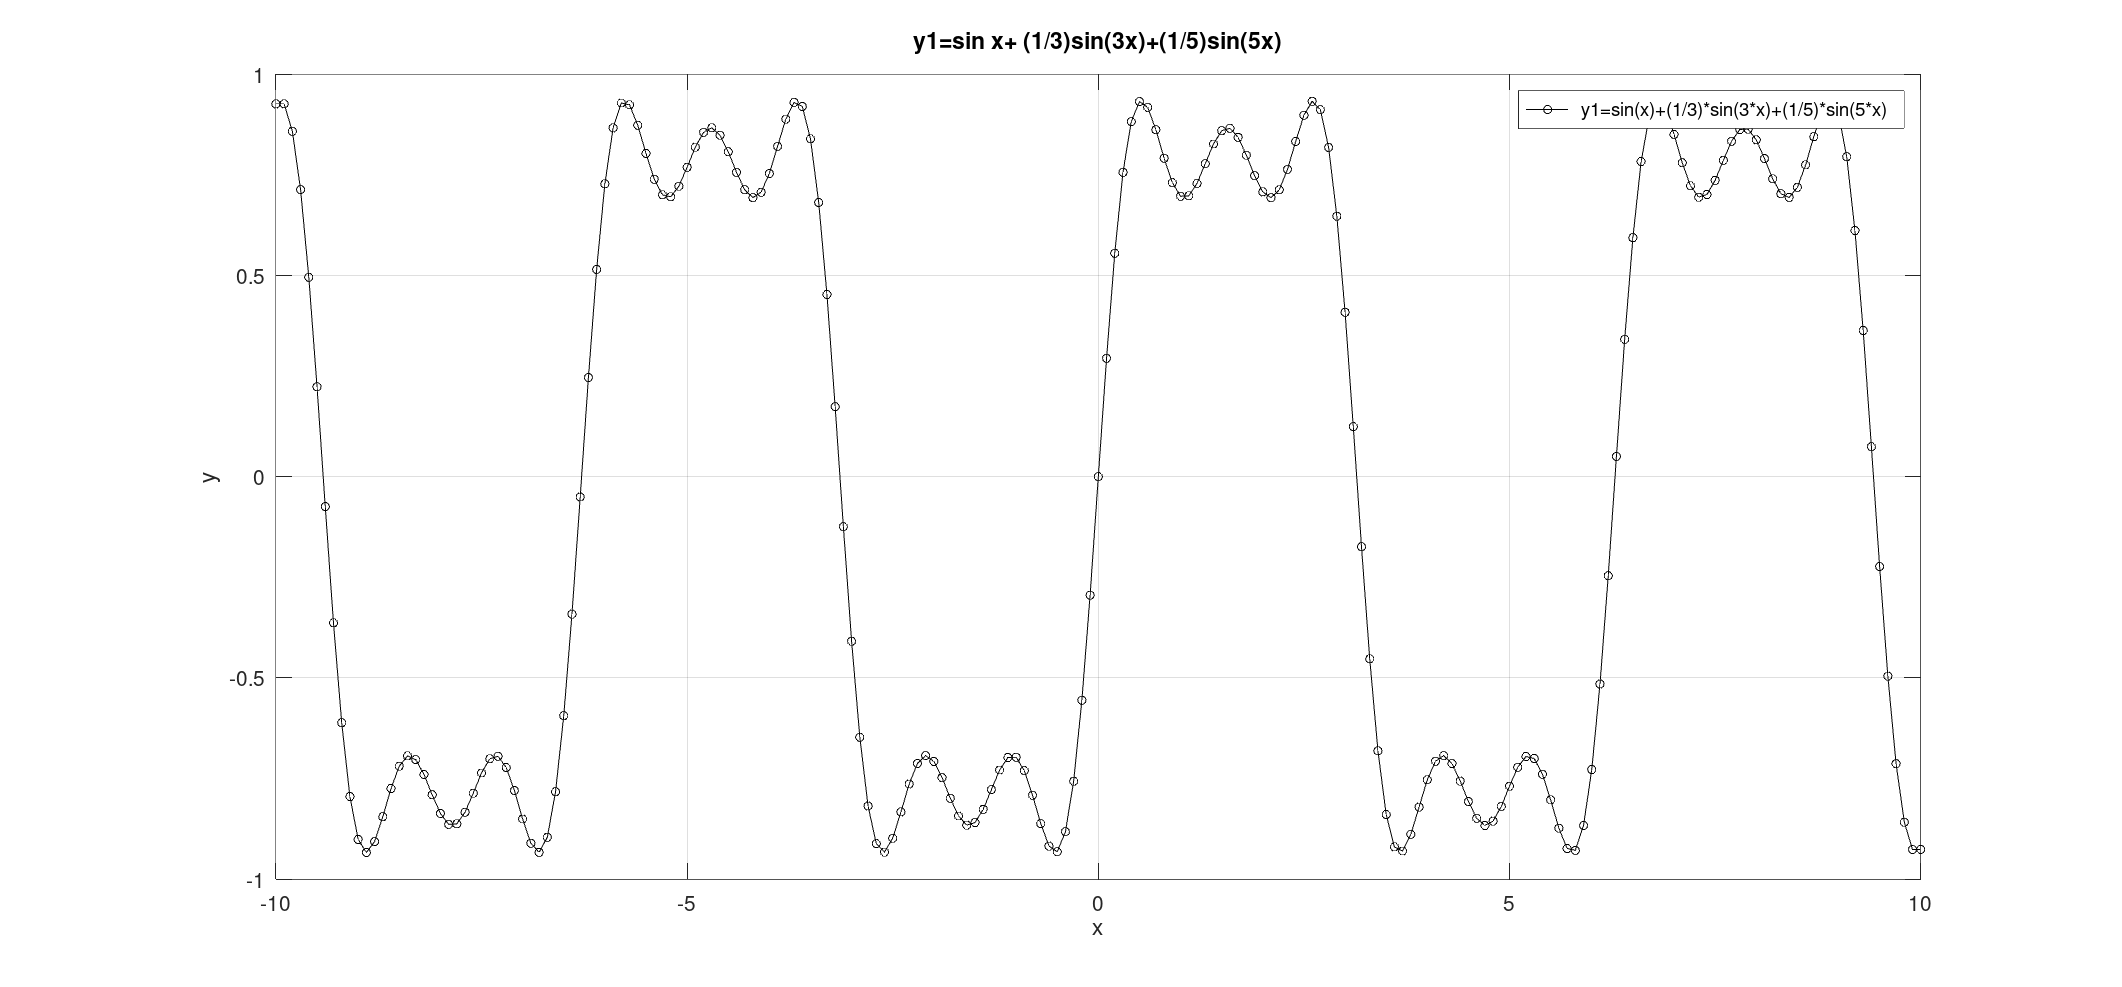
\includegraphics[width=\textwidth]{../octave/plot-sin.png}
            \captionof{figure}{График функции \(y = \sin{x} + \frac{1}{3} \sin{3x} + \frac{1}{5} \sin{5x} \)
        на интервале \([-10;10]\)}
            \label{img:plotsin}
        \end{center}

    \item В новом файле \texttt{plot\_sin\_cos.m} реализовали программу, которая строит
        на одном графике две линии, соответствующие функциям \(y1 = \sin{x} + \frac{1}{3} \sin{3x} + \frac{1}{5} \sin{5x}, y2 = \cos{x} + \frac{1}{3} \cos`{3x} + \frac{1}{5} \cos{5x}\):
        \begin{minted}{octave}
% Формирование массива x:
x=-10:0.1:10;
% Формирование массива y.
y1=sin(x)+1/3*sin(3*x)+1/5*sin(5*x);
y2=cos(x)+1/3*cos(3*x)+1/5*cos(5*x);
% Построение графика функции:
plot(x,y1,"-ok; y1=sin(x)+(1/3)*sin(3*x)+(1/5)*sin(5*x);","markersize",4, x, y2, "; y2=cos(x)+(1/3)*cos(3*x)+(1/5)*cos(5*x);")
% Отображение сетки на графике
grid on;
% Подпись оси X:
xlabel('x');
% Подпись оси Y:
ylabel('y');
% Название графика:
title('y1=sin x+ (1/3)sin(3x)+(1/5)sin(5x); y2=cos x+(1/3)cos(3x)+(1/5)cos(5x)');
% Экспорт рисунка в файл .eps:
print ("plot-sincos.eps", "-mono", "-FArial:16", "-deps")
% Экспорт рисунка в файл .png:
print("plot-sincos.png");
        \end{minted}

    \item В результате выполнения скрипта получен график, изображенный на Рисунке \ref{img:plotsincos}:
        \begin{center}
            \centering
            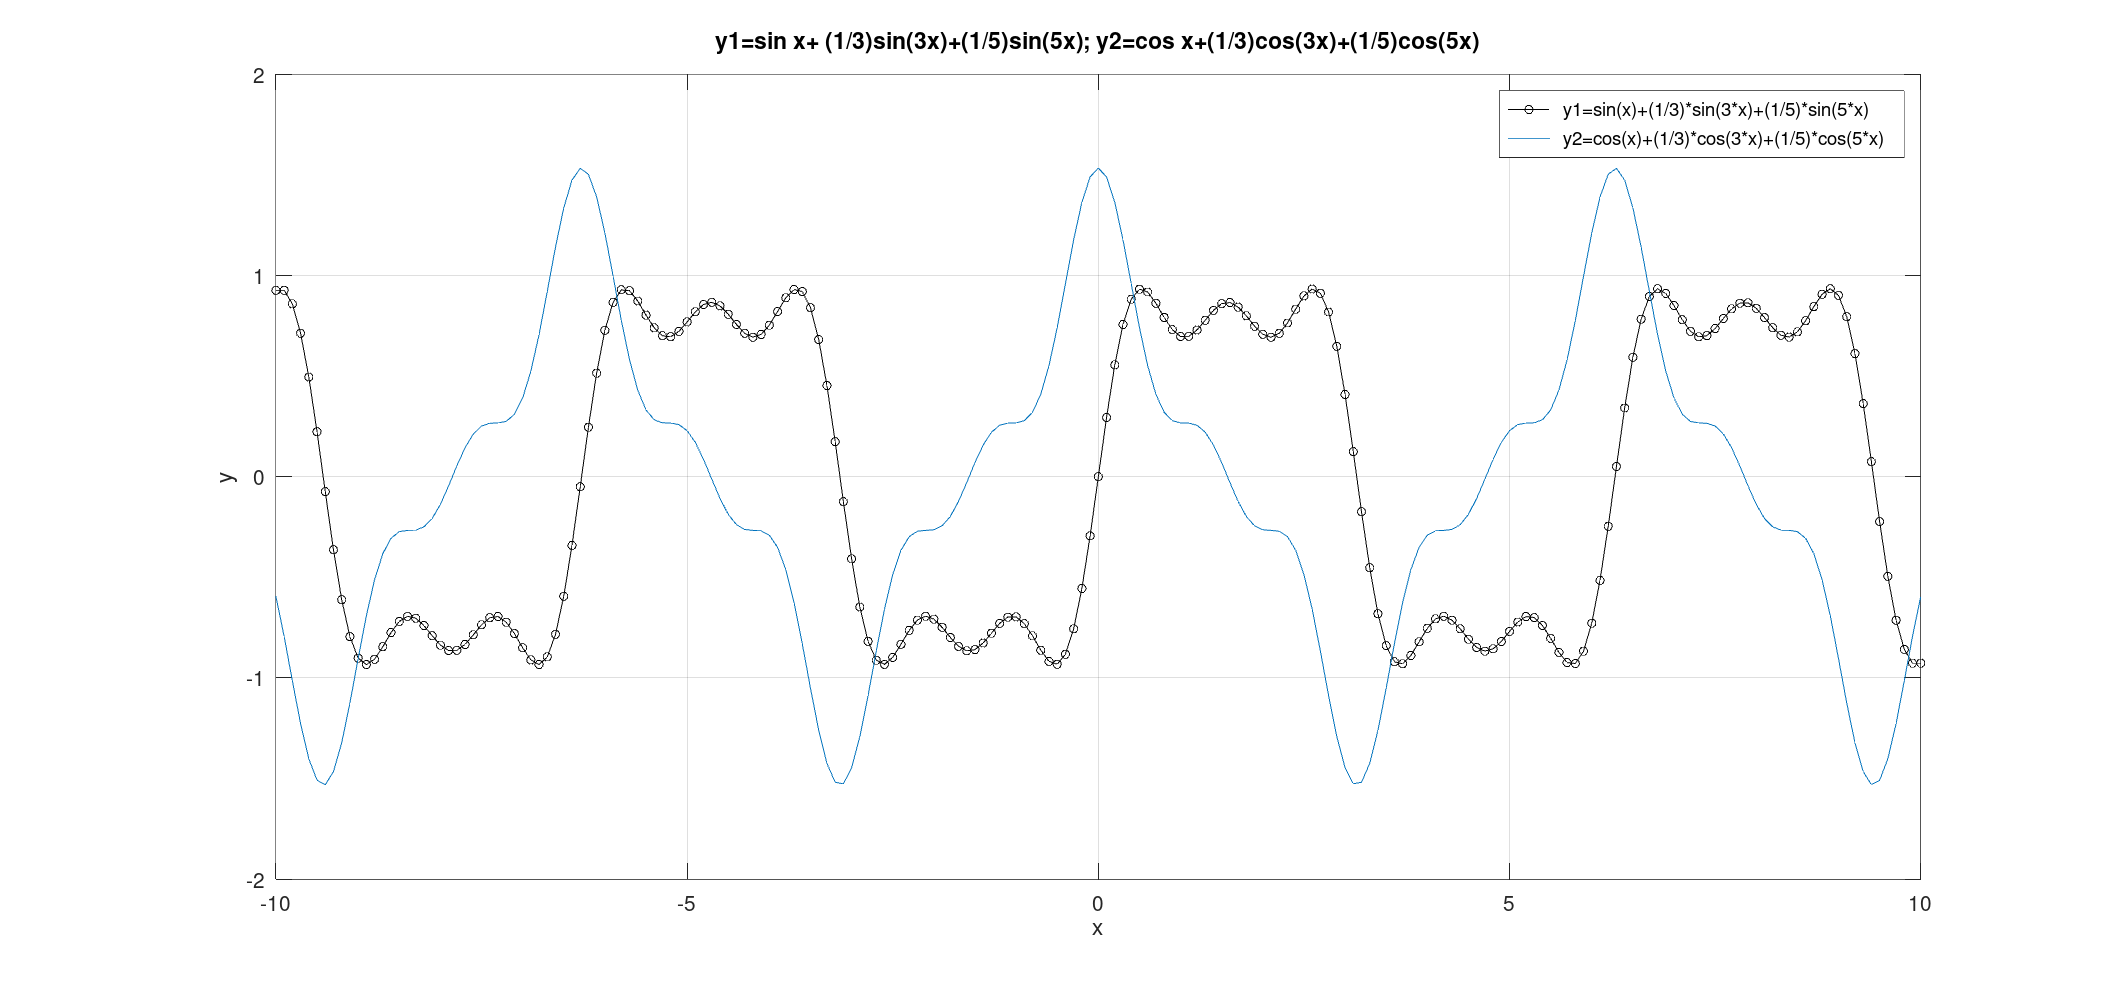
\includegraphics[width=\textwidth]{../octave/plot-sincos.png}
            \captionof{figure}{График функций \(y1 = \sin{x} + \frac{1}{3} \sin{3x} + \frac{1}{5} \sin{5x},y2 = \cos{x} + \frac{1}{3} \cos`{3x} + \frac{1}{5} \cos{5x} \)
        на интервале \([-10;10]\)}
            \label{img:plotsincos}
        \end{center}
\end{enumerate}

\subsection{Разложение импульсного сигнала в частичный ряд Фурье}

\begin{enumerate}
    \item Создали новый файл \texttt{meandr\_sin.m}, в котором реализовали программу,
        которая строит графики меандра с разными числом гармоник, используя синусы
        (Рисунок \ref{img:meandr-sin}). Листинг программы представлен ниже:
        \begin{minted}{octave}
% meandr.m
% количество отсчетов (гармоник):
N=8;
% частота дискретизации:
t=-1:0.01:1;
% значение амплитуды
A=1;
% период:
T=1;
% амплитуда гармоник
nh=(1:N)*2-1;
% массив коэффициентов для ряда, заданного через cos:
Am=2/pi ./ nh;
%Am(2:2:end) = -Am(2:2:end);
% массив гармоник:
harmonics=sin(2 * pi * nh' * t/T);
% массив элементов ряда:
s1=harmonics.*repmat(Am',1,length(t));
% Суммирование ряда:
s2=cumsum(s1);
% Построение графиков:
for k=1:N
  subplot(4,2,k)
  plot(t, s2(k,:))
  xticks(-1:.5:1)
  yticks(-1:.5:1)
end
% Экспорт рисунка в файл .png:
print("plot-meandr-sin.png");
        \end{minted}

        \begin{center}
            \centering
            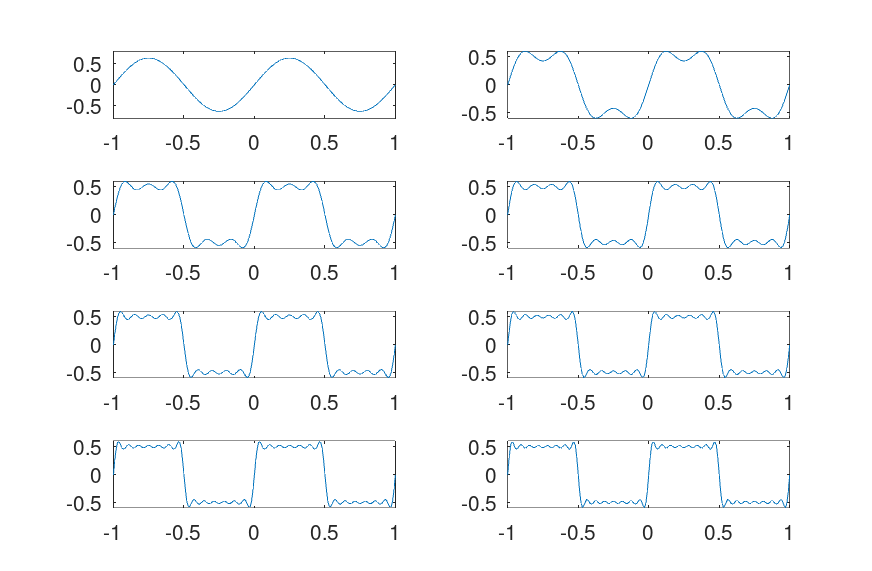
\includegraphics[width=\textwidth]{../octave/plot-meandr-sin.png}
            \captionof{figure}{Графики меандра, с различным числом гармоник (синусы).}
            \label{img:meandr-sin}
        \end{center}

    \item Создали новый файл \texttt{meandr\_cos.m}, в котором реализовали программу,
        которая строит графики меандра с разными числом гармоник, используя косинусы
        (Рисунок \ref{img:meandr-cos}). Листинг программы представлен ниже:
        \begin{minted}{octave}
% meandr.m
% количество отсчетов (гармоник):
N=8;
% частота дискретизации:
t=-1:0.01:1;
% значение амплитуды
A=1;
% период:
T=1;

% амплитуда гармоник
nh=(1:N)*2-1;
% массив коэффициентов для ряда, заданного через cos:
Am=2/pi ./ nh;
Am(2:2:end) = -Am(2:2:end);
% массив гармоник:
harmonics=cos(2 * pi * nh' * t/T);
% массив элементов ряда:
s1=harmonics.*repmat(Am',1,length(t))
% Суммирование ряда:
s2=cumsum(s1);
% Построение графиков:
for k=1:N
  subplot(4,2,k)
  plot(t, s2(k,:))
  xticks(-1:.5:1)
  yticks(-1:.5:1)
end

% Экспорт рисунка в файл .png:
print("plot-meandr-cos.png");
        \end{minted}

        \begin{center}
            \centering
            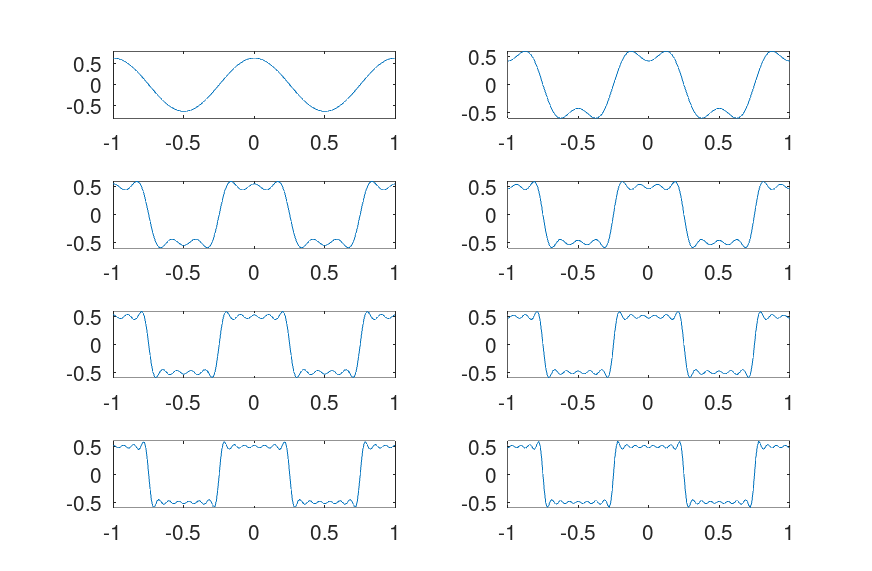
\includegraphics[width=\textwidth]{../octave/plot-meandr-cos.png}
            \captionof{figure}{графики меандра, с различным числом гармоник (косинусы).}
            \label{img:meandr-cos}
        \end{center}
\end{enumerate}

\subsection{Определение спектра и параметров сигнала}
\begin{enumerate}
    \item Создали каталог \texttt{spectre1} и в нем файл \texttt{spectre.m}.
        В файле реализовали программу, которая строит график с двумя сигналами
        разной частоты, затем с помощью быстрого преобразования Фурье находит спектры
        этих сигналов (Рисунки \ref{img:signal}-\ref{img:spectre-fix})

        \begin{minted}{octave}
% spectre1/spectre.m
% Создание каталогов signal и spectre для размещения графиков:
mkdir 'signal';
mkdir 'spectre';
% Длина сигнала (с):
tmax = 0.5;
% Частота дискретизации (Гц) (количество отсчётов):
fd = 512;
% Частота первого сигнала (Гц):
f1 = 10;
% Частота второго сигнала (Гц):
f2 = 40;
% Амплитуда первого сигнала:
a1 = 1;
% Амплитуда второго сигнала:
a2 = 0.7;
% Массив отсчётов времени:
t = 0:1./fd:tmax;
% Спектр сигнала:
fd2 = fd/2;

% Два сигнала разной частоты:
signal1 = a1*sin(2*pi*t*f1);
signal2 = a2*sin(2*pi*t*f2);

% График 1-го сигнала:
plot(signal1,'b');
% График 2-го сигнала:
hold on
plot(signal2,'r');
hold off
title('Signal');
% Экспорт графика в файл в каталоге signal:
print 'signal/spectre.png';

% Посчитаем спектр
% Амплитуды преобразования Фурье сигнала 1:
spectre1 = abs(fft(signal1,fd));
% Амплитуды преобразования Фурье сигнала 2:
spectre2 = abs(fft(signal2,fd));
% Построение графиков спектров сигналов:
plot(spectre1,'b');
hold on
plot(spectre2,'r');
hold off
title('Spectre');
print 'spectre/spectre.png';

% Исправление графика спектра
% Сетка частот:
f = 1000*(0:fd2)./(2*fd);
% Нормировка спектров по амплитуде:
spectre1 = 2*spectre1/fd2;
spectre2 = 2*spectre2/fd2;
% Построение графиков спектров сигналов:
plot(f,spectre1(1:fd2+1),'b');
hold on
plot(f,spectre2(1:fd2+1),'r');
hold off
xlim([0 100]);
title('Fixed spectre');
xlabel('Frequency (Hz)');
print 'spectre/spectre_fix.png';
        \end{minted}

        \begin{center}
            \centering
            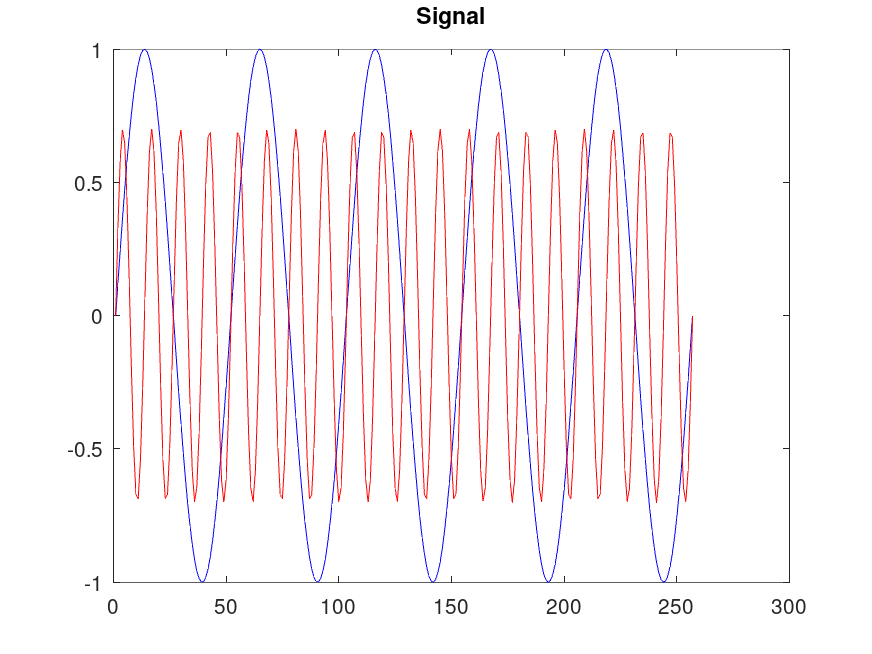
\includegraphics[width=\textwidth]{../octave/spectre1/signal/spectre.png}
            \captionof{figure}{Два синусоидальных сигнала разной частоты.}
            \label{img:signal}
        \end{center}
        \begin{center}
            \centering
            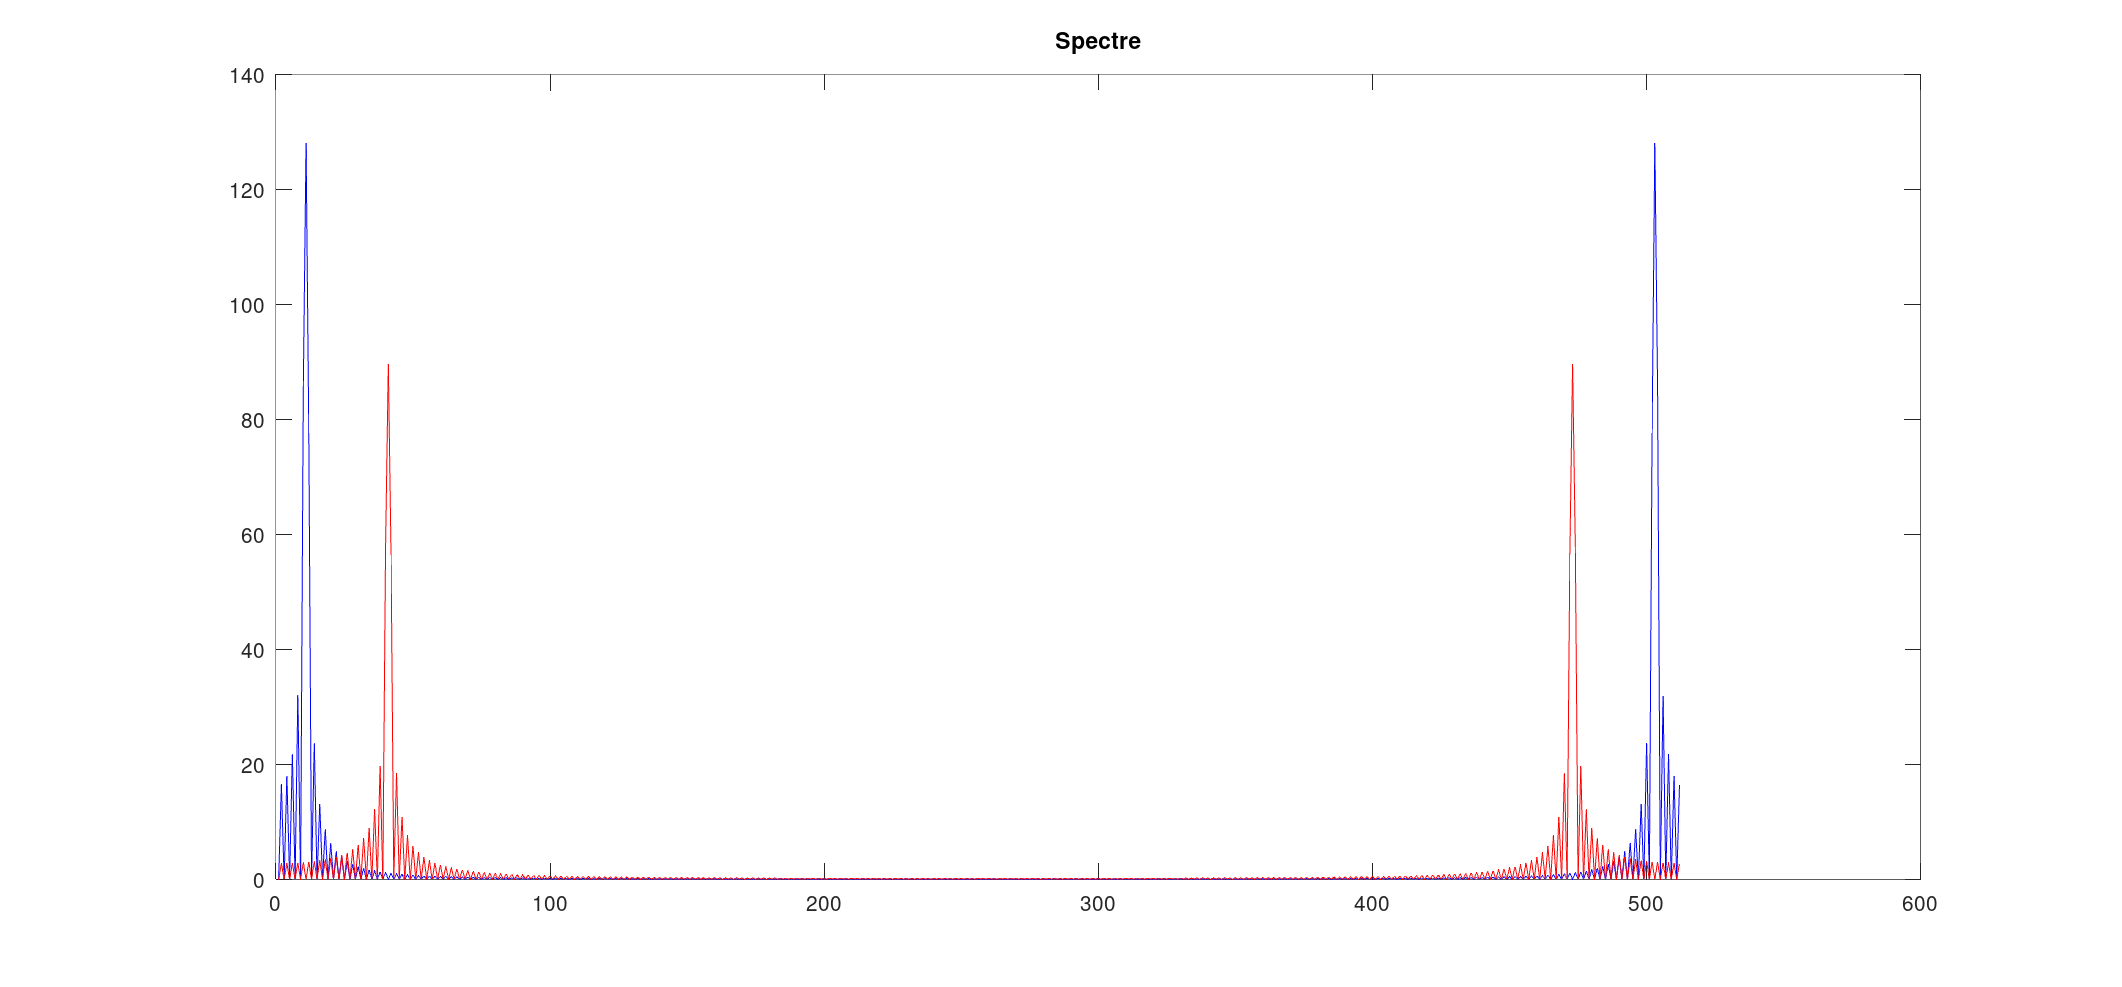
\includegraphics[width=\textwidth]{../octave/spectre1/spectre/spectre.png}
            \captionof{figure}{График спектров синусоидальных сигналов.}
            \label{img:spectre}
        \end{center}
        \begin{center}
            \centering
            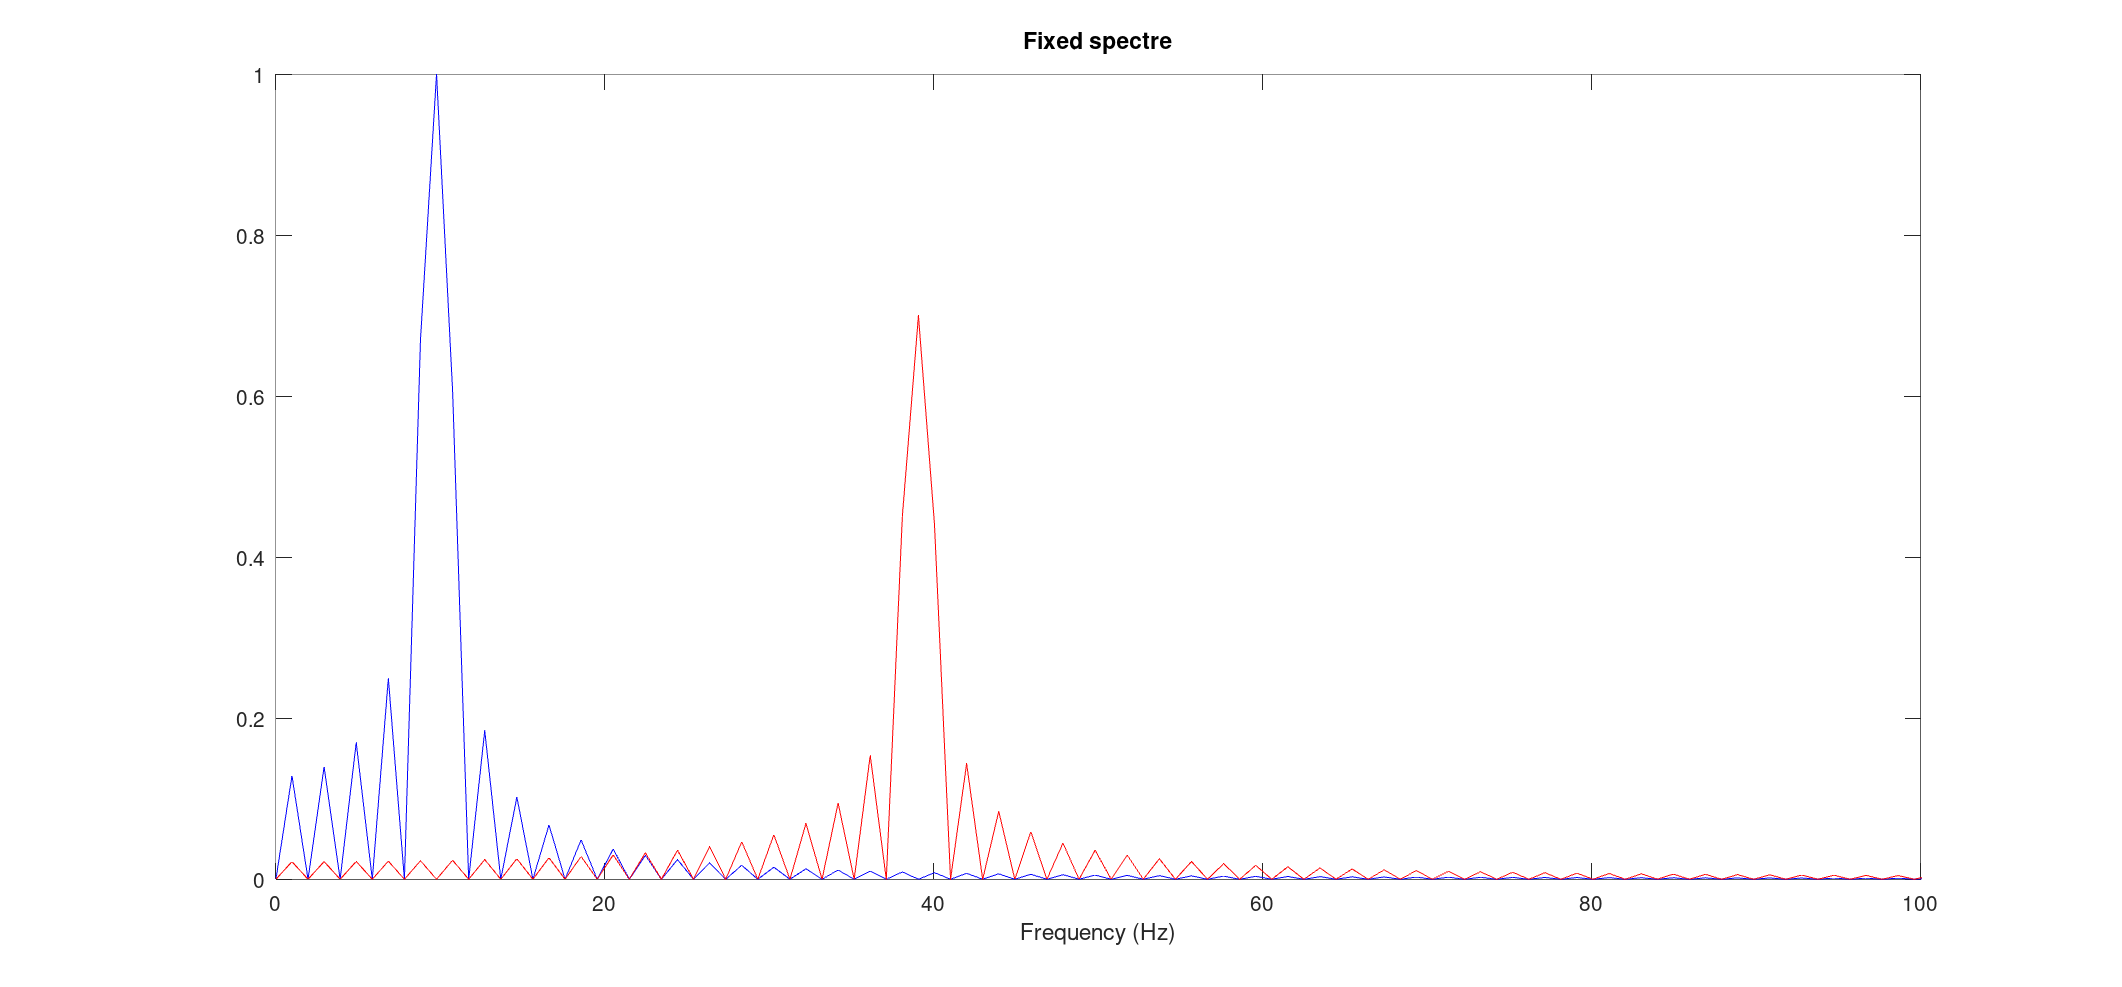
\includegraphics[width=\textwidth]{../octave/spectre1/spectre/spectre_fix.png}
            \captionof{figure}{Исправленный график спектров синусоидальных сигналов.}
            \label{img:spectre-fix}
        \end{center}
\end{enumerate}

\subsection{Амплитудная модуляция}
\begin{enumerate}
    \item Создали каталог \texttt{modulation} и в нем файл \texttt{am.m}.
        В файле реализовали программу, которая определяет спектр сигнала при
        амплитудной модуляции и строит соответствующие графики
        (Рисунки \ref{img:modulation-signal}, \ref{img:modulation-spectre}):

        \begin{minted}{octave}
% modulation/am.m
% Создание каталогов signal и spectre для размещения графиков:
mkdir 'signal';
mkdir 'spectre';
% Модуляция синусоид с частотами 50 и 5
% Длина сигнала (с)
tmax = 0.5;
% Частота дискретизации (Гц) (количество отсчётов)
fd = 512;
% Частота сигнала (Гц)
f1 = 5;
% Частота несущей (Гц)
f2 = 50;
% Спектр сигнала
fd2 = fd/2;
% Построение графиков двух сигналов (синусоиды)
% разной частоты
% Массив отсчётов времени:
t = 0:1./fd:tmax;
signal1 = sin(2*pi*t*f1);
signal2 = sin(2*pi*t*f2);
signal = signal1 .* signal2;
plot(signal, 'b');
hold on
% Построение огибающей:
plot(signal1, 'r');
plot(-signal1, 'r');
hold off
title('Signal');
print 'signal/am.png';
% Расчет спектра:
% Амплитуды преобразования Фурье-сигнала:
spectre = fft(signal,fd);
% Сетка частот:
f = 1000*(0:fd2)./(2*fd);
% Нормировка спектра по амплитуде:
spectre = 2*sqrt(spectre.*conj(spectre))./fd2;
% Построение спектра:
plot(f,spectre(1:fd2+1), 'b')
xlim([0 100]);
title('Spectre');
xlabel('Frequency (Hz)');
print 'spectre/am.png';
        \end{minted}

        \begin{center}
            \centering
            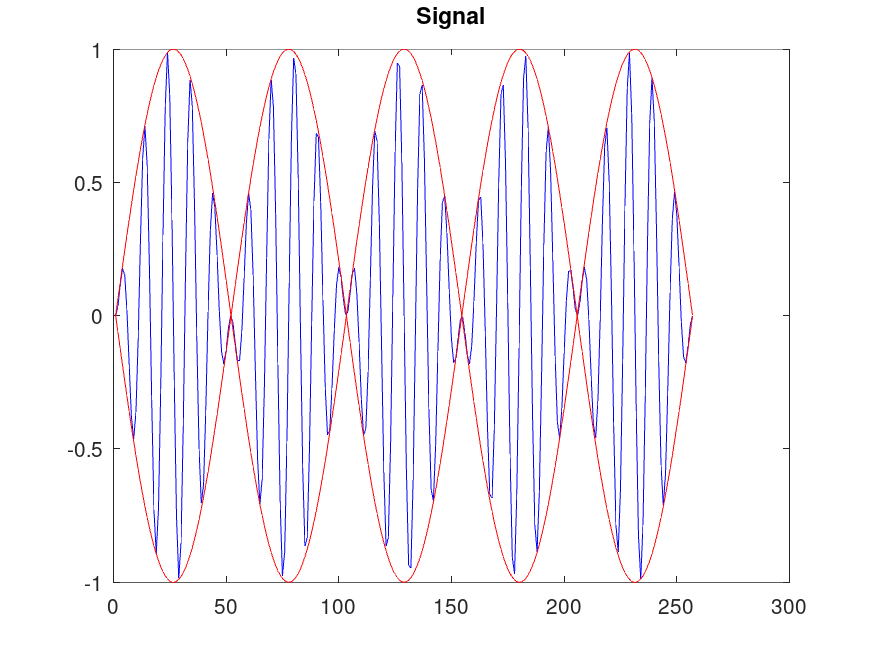
\includegraphics[width=\textwidth]{../octave/modulation/signal/am.png}
            \captionof{figure}{Сигнал и огибающая при амплитудной модуляции.}
            \label{img:modulation-signal}
        \end{center}
        \begin{center}
            \centering
            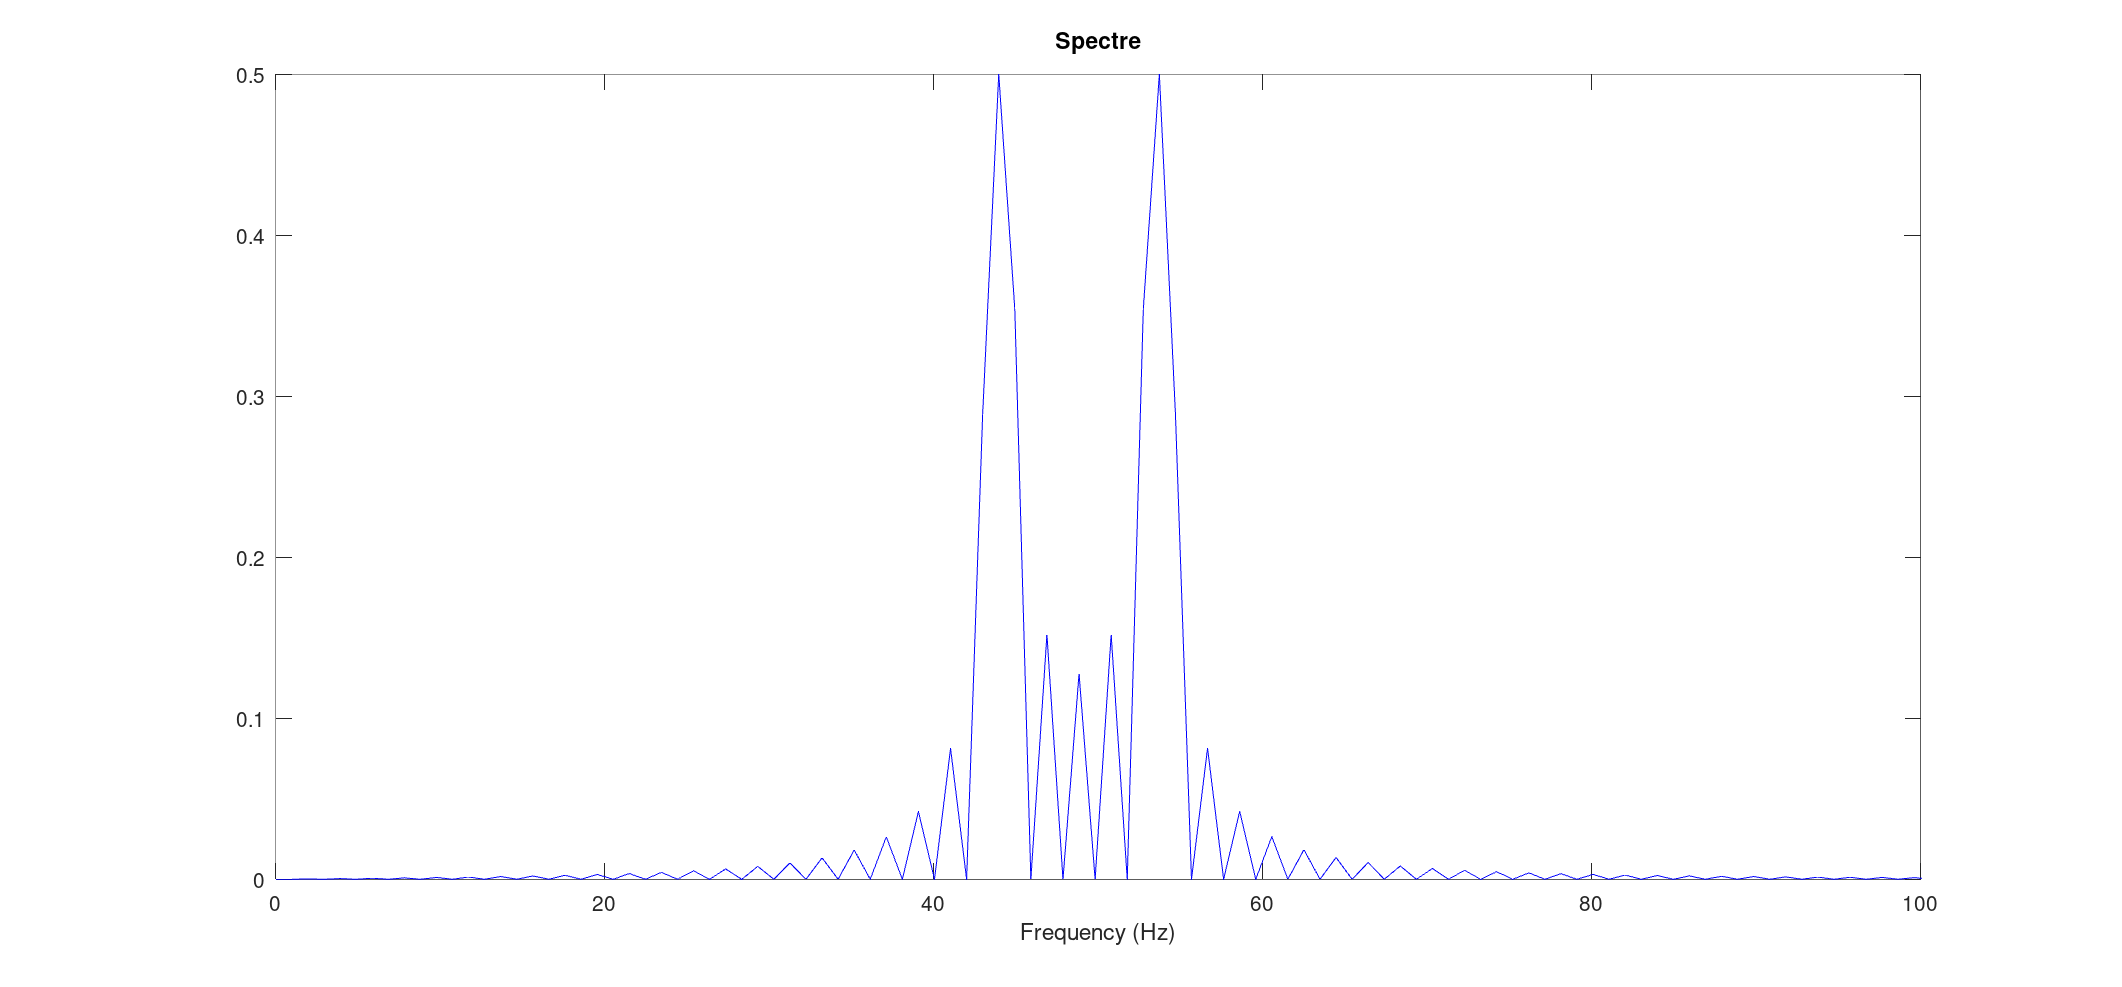
\includegraphics[width=\textwidth]{../octave/modulation/spectre/am.png}
            \captionof{figure}{Спектр сигнала при амплитудной модуляции.}
            \label{img:modulation-spectre}
        \end{center}
\end{enumerate}

\subsection{Кодирование сигнала. Исследование свойства самосинхронизации сигнала}
\begin{enumerate}
    \item Создали каталог \texttt{coding} и в нем файлы: \texttt{main.m},
        \texttt{maptowave.m}, \texttt{unipolar.m}, \texttt{ami.m},
        \texttt{bipolarnrz.m}, \texttt{bipolarrz.m}, \texttt{manchester.m},
        \texttt{diffmanc.m}, \texttt{calcspectre.m}.
    \item Листинги каждого файла приведены ниже:
        \begin{itemize}
        \item В файле \texttt{maptowave.m}:
            \begin{minted}{octave}
% coding/maptowave.m
function wave=maptowave(data)
  data=upsample(data,100);
  wave=filter(5*ones(1,100),1,data);
            \end{minted}
        \item В файле \texttt{unipolar.m}:
            \begin{minted}{octave}
% coding/unipolar.m
% Униполярное кодирование:
function wave=unipolar(data)
  wave=maptowave(data)
            \end{minted}
        \item В файле \texttt{ami.m}:
            \begin{minted}{octave}
% coding/ami.m
% Кодирование AMI:
function wave=ami(data)
  am=mod(1:length(data(data==1)),2);
  am(am==0)=-1;
  data(data==1)=am;
  wave=maptowave(data);
            \end{minted}
        \item В файле \texttt{bipolarnrz.m}:
            \begin{minted}{octave}
% coding/bipolarnrz.m
% Кодирование NRZ:
function wave=bipolarnrz(data)
  data(data==0)=-1;
  wave=maptowave(data);
            \end{minted}
        \item В файле \texttt{bipolarrz.m}:
            \begin{minted}{octave}
% coding/bipolarrz.m
% Кодирование RZ:
function wave=bipolarrz(data)
  data(data==0)=-1;
  data=upsample(data,2);
  wave=maptowave(data);
            \end{minted}
        \item В файле \texttt{manchester.m}:
            \begin{minted}{octave}
% coding/manchester.m
% Манчестерское кодирование:
function wave=manchester(data)
  data(data==0)=-1;
  data=upsample(data,2);
  data=filter([-1 1],1,data);
  wave=maptowave(data);
            \end{minted}
        \item В файле \texttt{diffmanc.m}:
            \begin{minted}{octave}
% coding/diffmanc.m
% Дифференциальное манчестерское кодирование
function wave=diffmanc(data)
  data=filter(1,[1 1],data);
  data=mod(data,2);
  wave=manchester(data);
            \end{minted}
        \item В файле \texttt{calcspectre.m}:
            \begin{minted}{octave}
% calcspectre.m
% Функция построения спектра сигнала:
function spectre = calcspectre(wave)
  % Частота дискретизации (Гц):
  Fd = 512;
  Fd2 = Fd/2;
  Fd3 = Fd/2 + 1;
  X = fft(wave,Fd);
  spectre = X.*conj(X)/Fd;
  f = 1000*(0:Fd2)/Fd;
  plot(f,spectre(1:Fd3));
  xlabel('Frequency (Hz)');
            \end{minted}
        \item В файле \texttt{main.m}:
            \begin{minted}{octave}
% coding/main.m
% Подключение пакета signal:
pkg load signal;
% Входная кодовая последовательность:
data=[0 1 0 0 1 1 0 0 0 1 1 0];
% Входная кодовая последовательность для проверки свойства самосинхронизации:
data_sync=[0 0 0 0 0 0 0 1 1 1 1 1 1 1];
% Входная кодовая последовательность для построения спектра сигнала:
data_spectre=[0 1 0 1 0 1 0 1 0 1 0 1 0 1];
% Создание каталогов signal, sync и spectre для размещения графиков:
mkdir 'signal';
mkdir 'sync';
mkdir 'spectre';
axis("auto");

% Униполярное кодирование
wave=unipolar(data);
plot(wave);
ylim([-1 6]);
title('Unipolar');
print 'signal/unipolar.png';
% Кодирование ami
wave=ami(data);
plot(wave)
title('AMI');
print 'signal/ami.png';
% Кодирование NRZ
wave=bipolarnrz(data);
plot(wave);
title('Bipolar Non-Return to Zero');
print 'signal/bipolarnrz.png';
% Кодирование RZ
wave=bipolarrz(data);
plot(wave)
title('Bipolar Return to Zero');
print 'signal/bipolarrz.png';
% Манчестерское кодирование
wave=manchester(data);
plot(wave)
title('Manchester');
print 'signal/manchester.png';
% Дифференциальное манчестерское кодирование
wave=diffmanc(data);
plot(wave)
title('Differential Manchester');
print 'signal/diffmanc.png';

% Униполярное кодирование
wave=unipolar(data_sync);
plot(wave);
ylim([-1 6]);
title('Unipolar');
print 'sync/unipolar.png';
% Кодирование AMI
wave=ami(data_sync);
plot(wave)
title('AMI');
print 'sync/ami.png';
% Кодирование NRZ
wave=bipolarnrz(data_sync);
plot(wave);
title('Bipolar Non-Return to Zero');
print 'sync/bipolarnrz.png';
% Кодирование RZ
wave=bipolarrz(data_sync);
plot(wave)
title('Bipolar Return to Zero');
print 'sync/bipolarrz.png';
% Манчестерское кодирование
wave=manchester(data_sync);
plot(wave)
title('Manchester');
print 'sync/manchester.png';
% Дифференциальное манчестерское кодирование
wave=diffmanc(data_sync);
plot(wave)
title('Differential Manchester');
print 'sync/diffmanc.png';

% Униполярное кодирование:
wave=unipolar(data_spectre);
spectre=calcspectre(wave);
title('Unipolar');
print 'spectre/unipolar.png';
% Кодирование AMI:
wave=ami(data_spectre);
spectre=calcspectre(wave);
title('AMI');
print 'spectre/ami.png';
% Кодирование NRZ:
wave=bipolarnrz(data_spectre);
spectre=calcspectre(wave);
title('Bipolar Non-Return to Zero');
print 'spectre/bipolarnrz.png';
% Кодирование RZ:
wave=bipolarrz(data_spectre);
spectre=calcspectre(wave);
title('Bipolar Return to Zero');
print 'spectre/bipolarrz.png';
% Манчестерское кодирование:
wave=manchester(data_spectre);
spectre=calcspectre(wave);
title('Manchester');
print 'spectre/manchester.png';
% Дифференциальное манчестерское кодирование:
wave=diffmanc(data_spectre);
spectre=calcspectre(wave);
title('Differential Manchester');
print 'spectre/diffmanc.png';
            \end{minted}
        \end{itemize}

    \item После запуска главного скрипта \texttt{main.m} получены файлы с графиками
        кодированного сигнала: графики кодированного сигнала
        (Рис. \ref{img:coding-sig-unipolar}-\ref{img:coding-sig-diffmanc}),
        графики, иллюстрирующие свойства самосинхронизации
        (Рис. \ref{img:coding-sync-unipolar}-\ref{img:coding-sync-diffmanc}),
        графики спектров сигналов
        (Рис. \ref{img:coding-spectre-unipolar}-\ref{img:coding-spectre-diffmanc}):
        \begin{center}
            \centering
            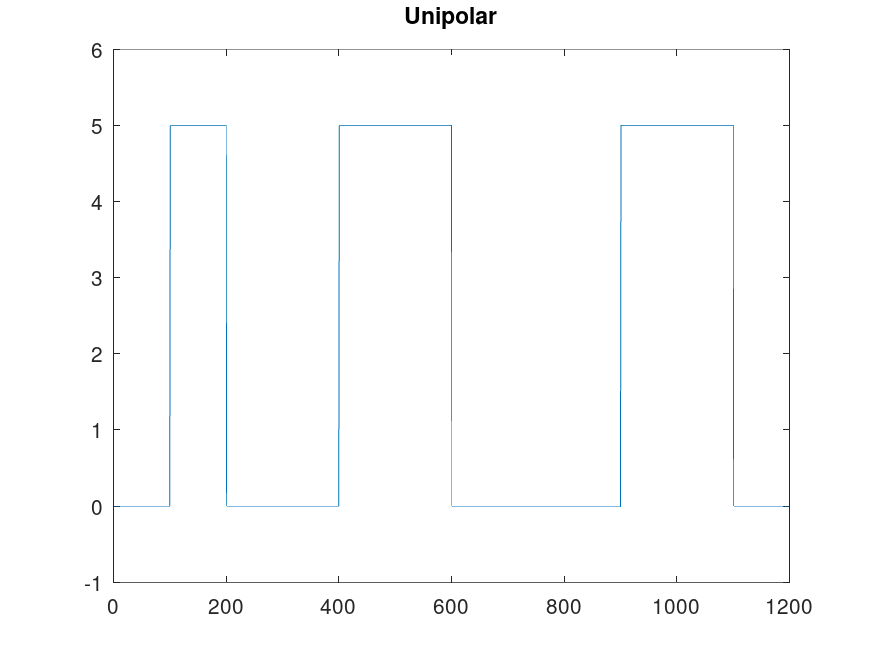
\includegraphics[width=0.7\textwidth]{../octave/coding/signal/unipolar.png}
            \captionof{figure}{Униполярное кодирование.}
            \label{img:coding-sig-unipolar}
        \end{center}
        \begin{center}
            \centering
            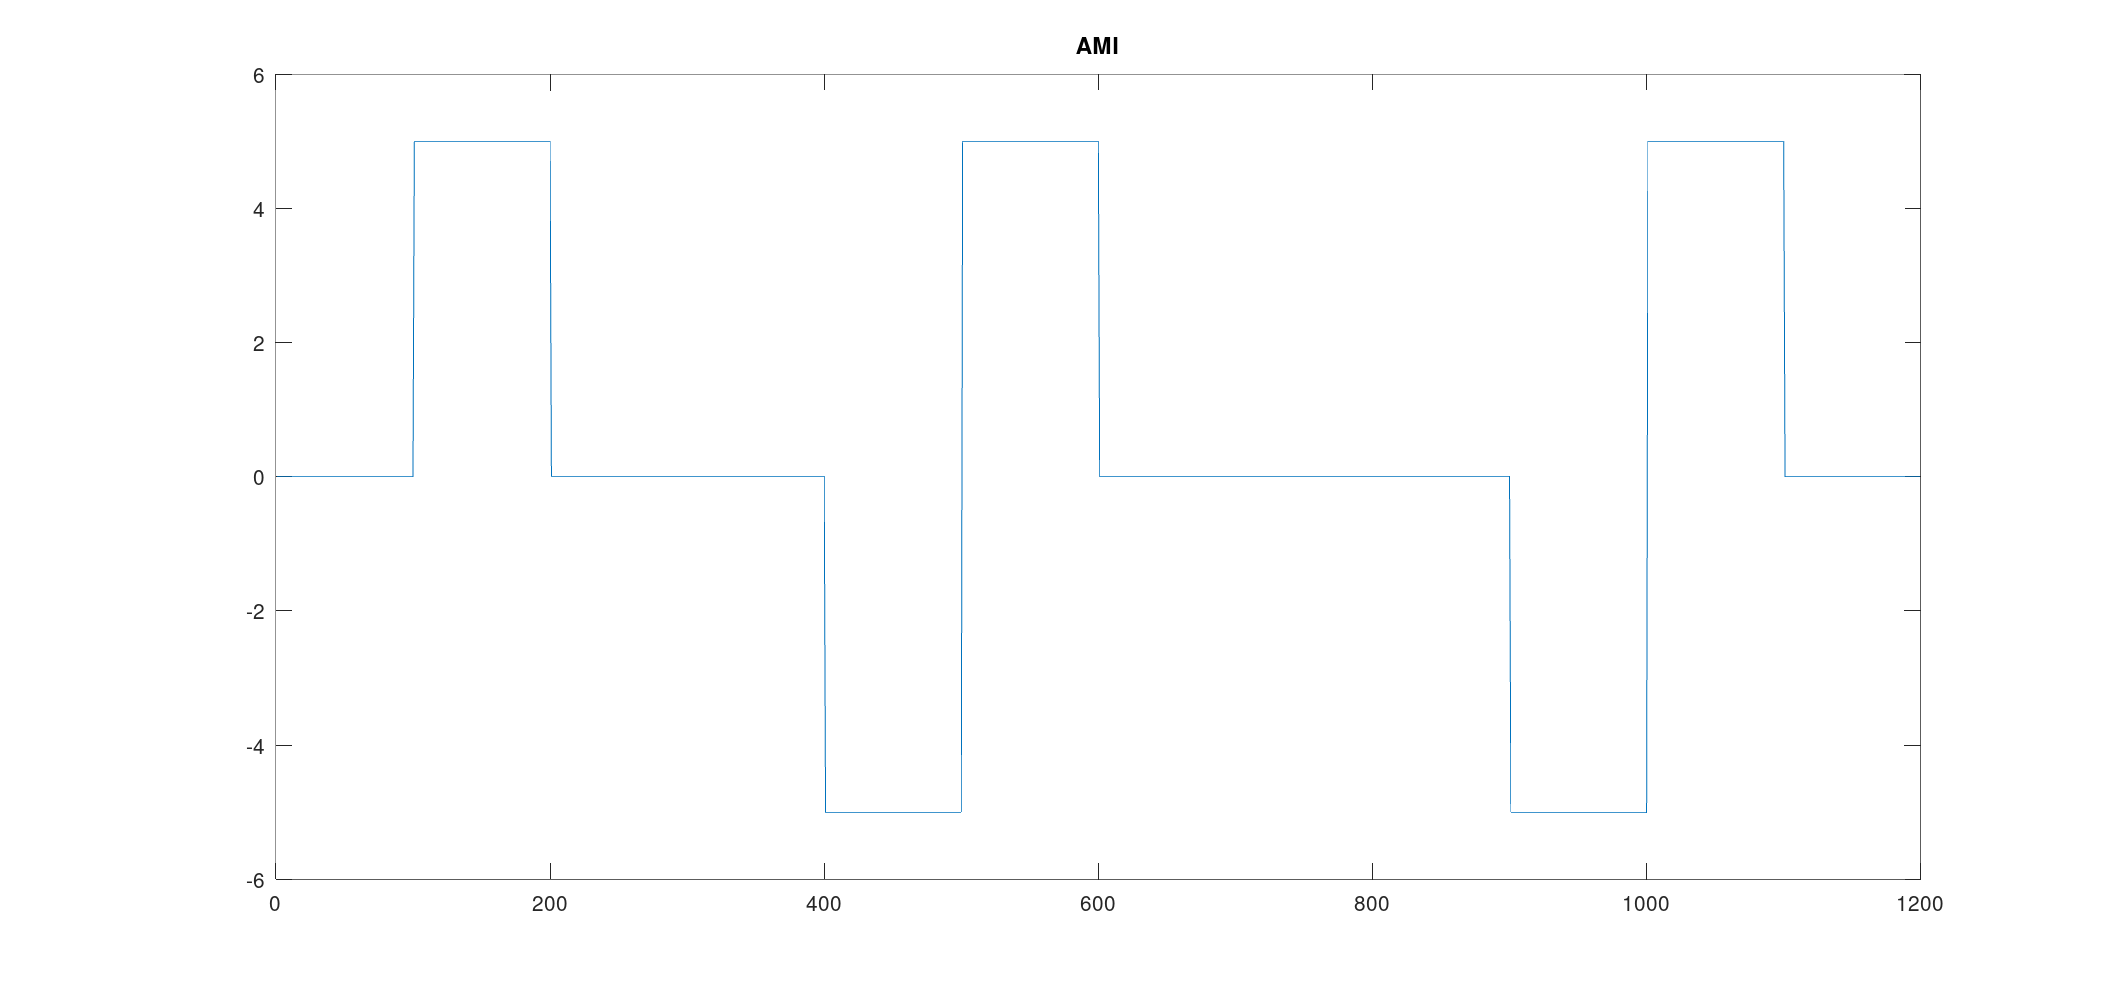
\includegraphics[width=0.7\textwidth]{../octave/coding/signal/ami.png}
            \captionof{figure}{Кодирование AMI.}
            \label{img:coding-sig-ami}
        \end{center}
        \begin{center}
            \centering
            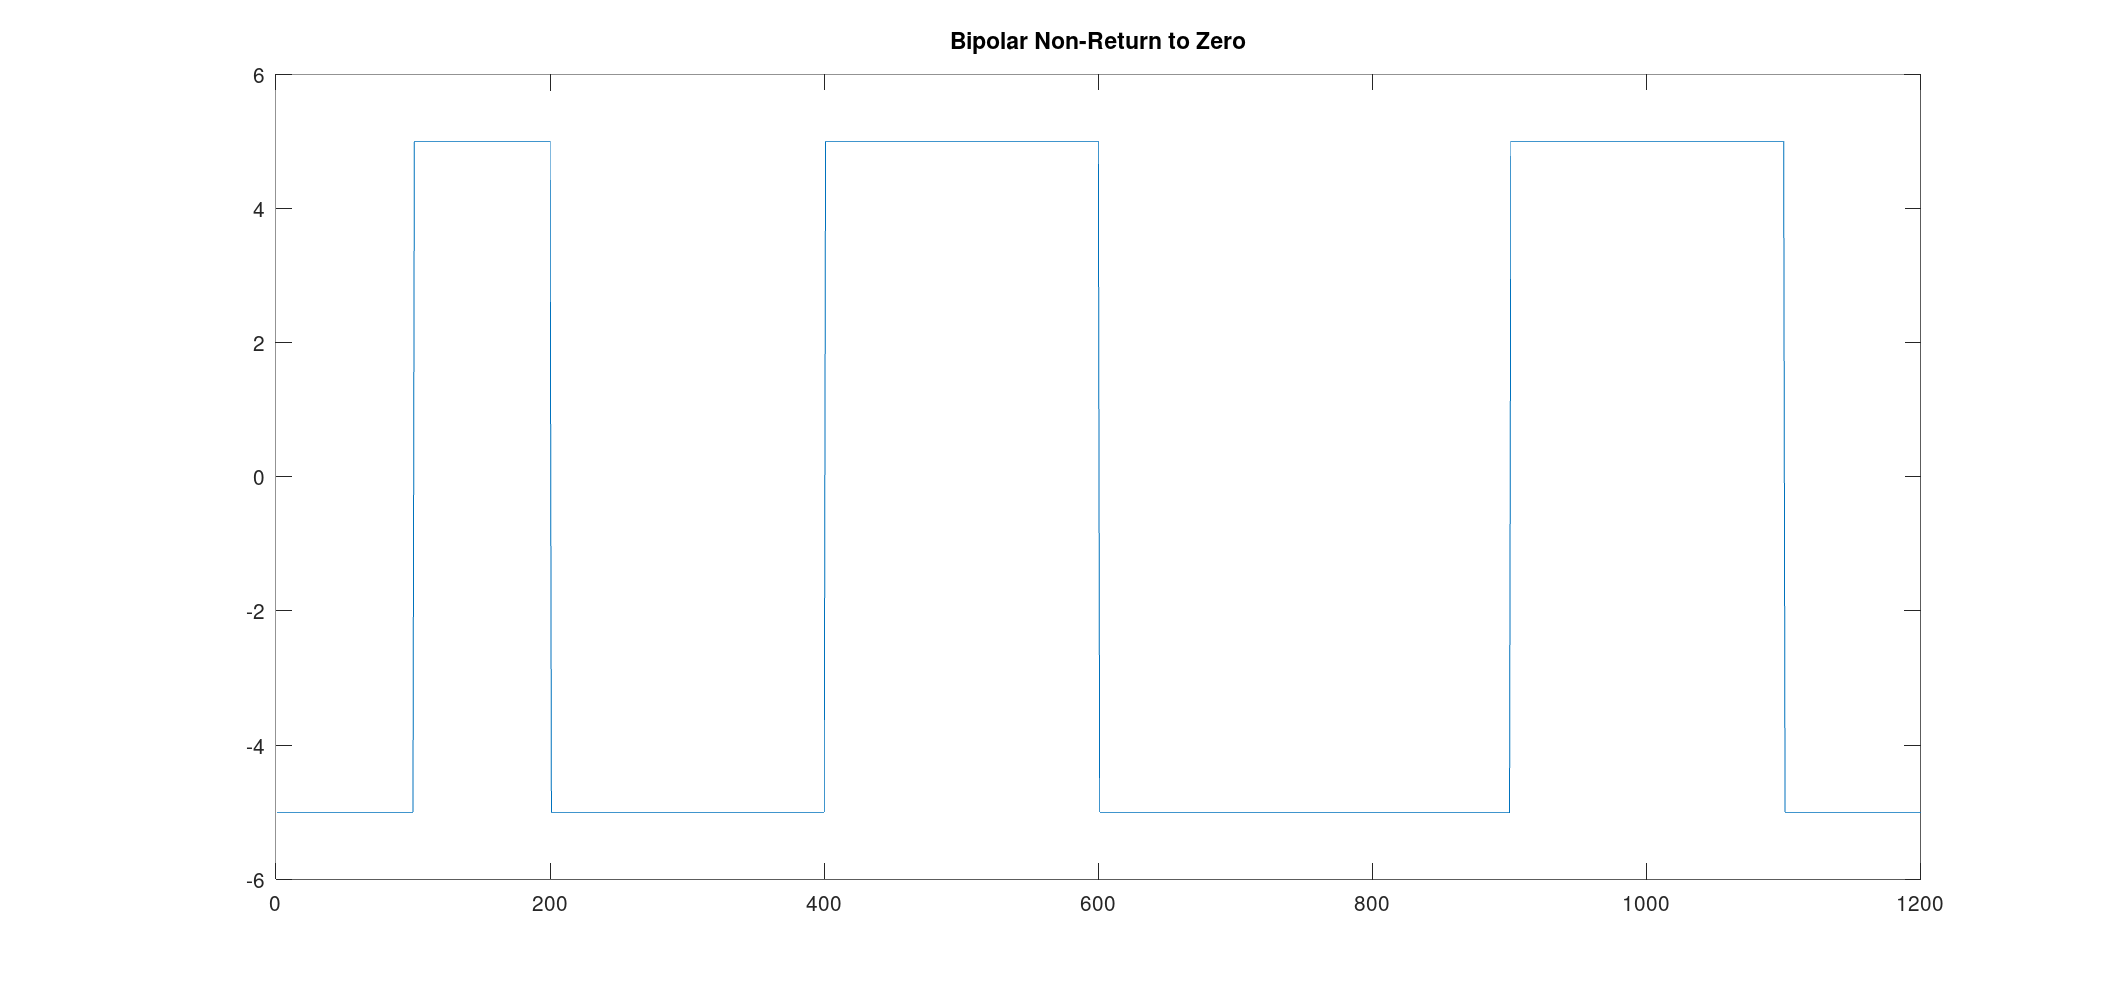
\includegraphics[width=0.7\textwidth]{../octave/coding/signal/bipolarnrz.png}
            \captionof{figure}{Кодирование NRZ}
            \label{img:coding-sig-nrz}
        \end{center}
        \begin{center}
            \centering
            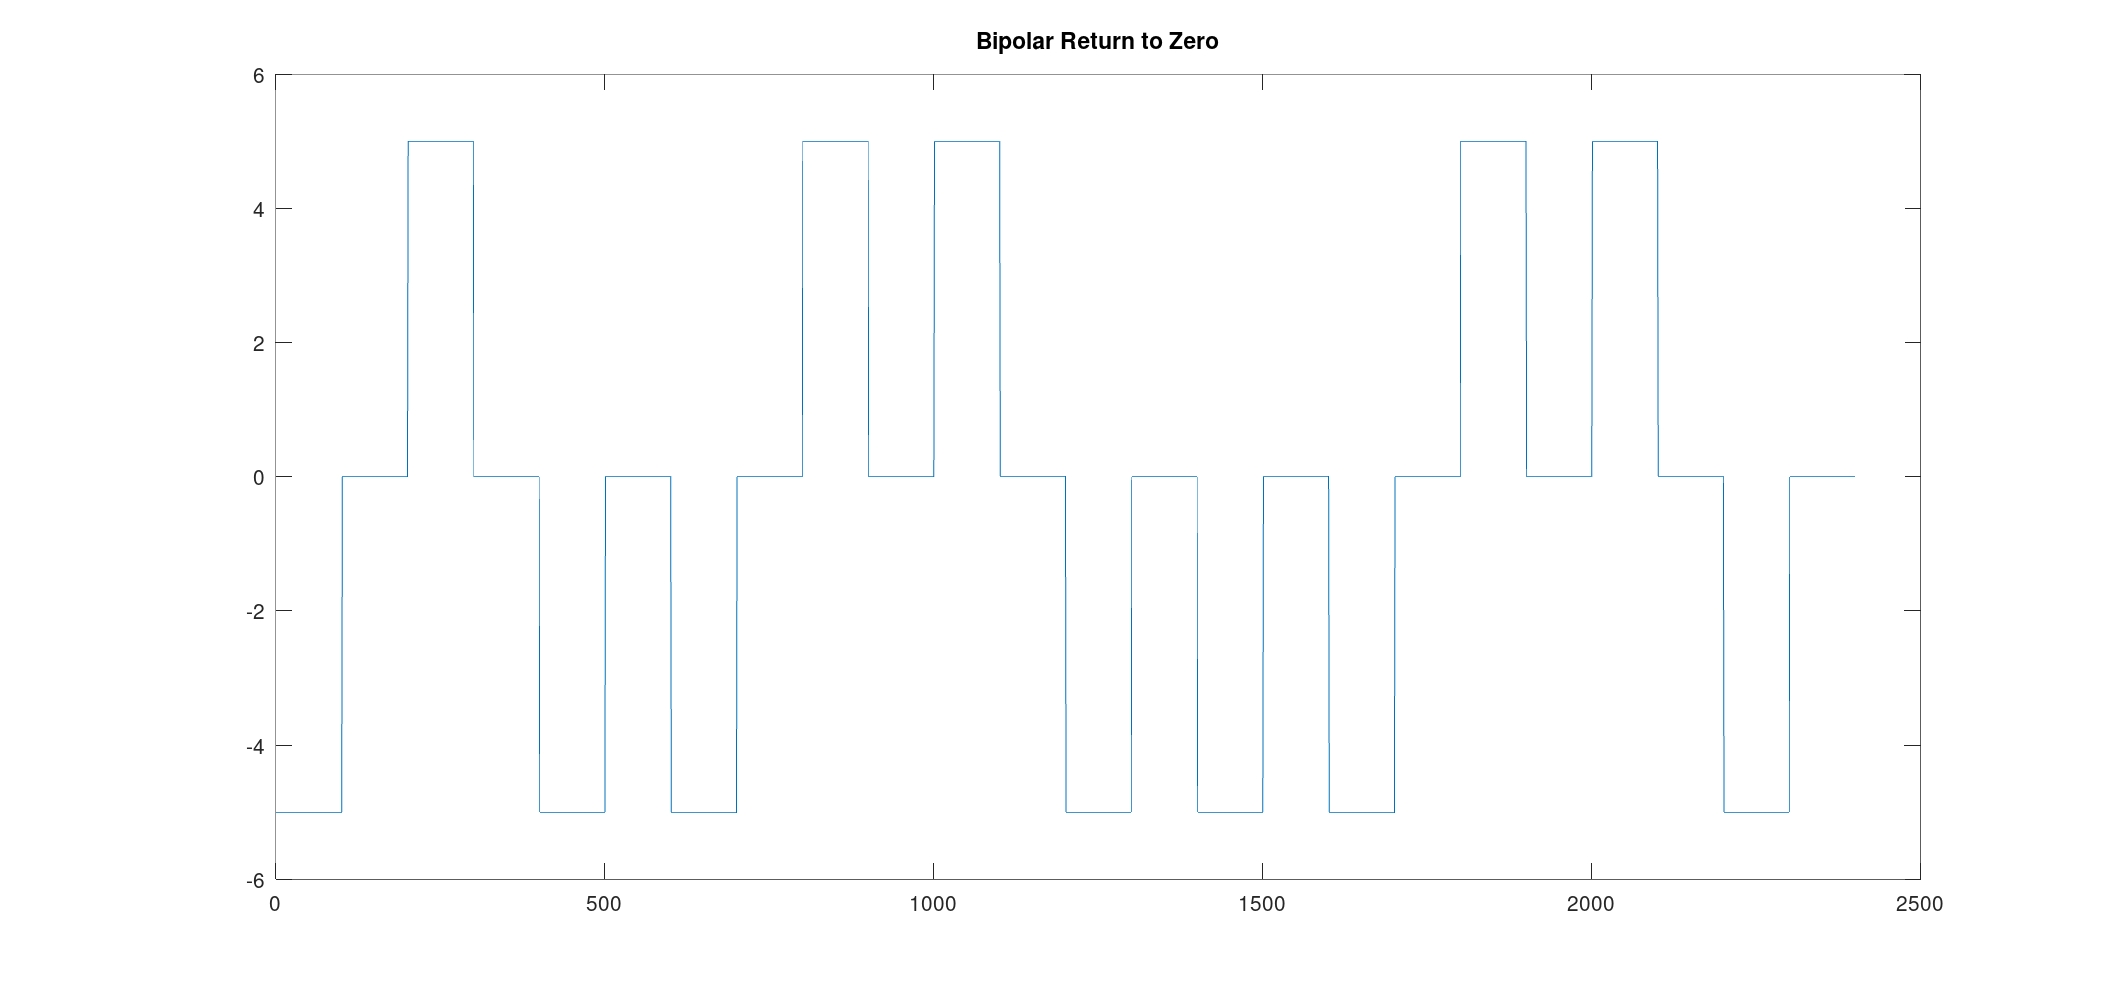
\includegraphics[width=0.7\textwidth]{../octave/coding/signal/bipolarrz.png}
            \captionof{figure}{Кодирование RZ}
            \label{img:coding-sig-rz}
        \end{center}
        \begin{center}
            \centering
            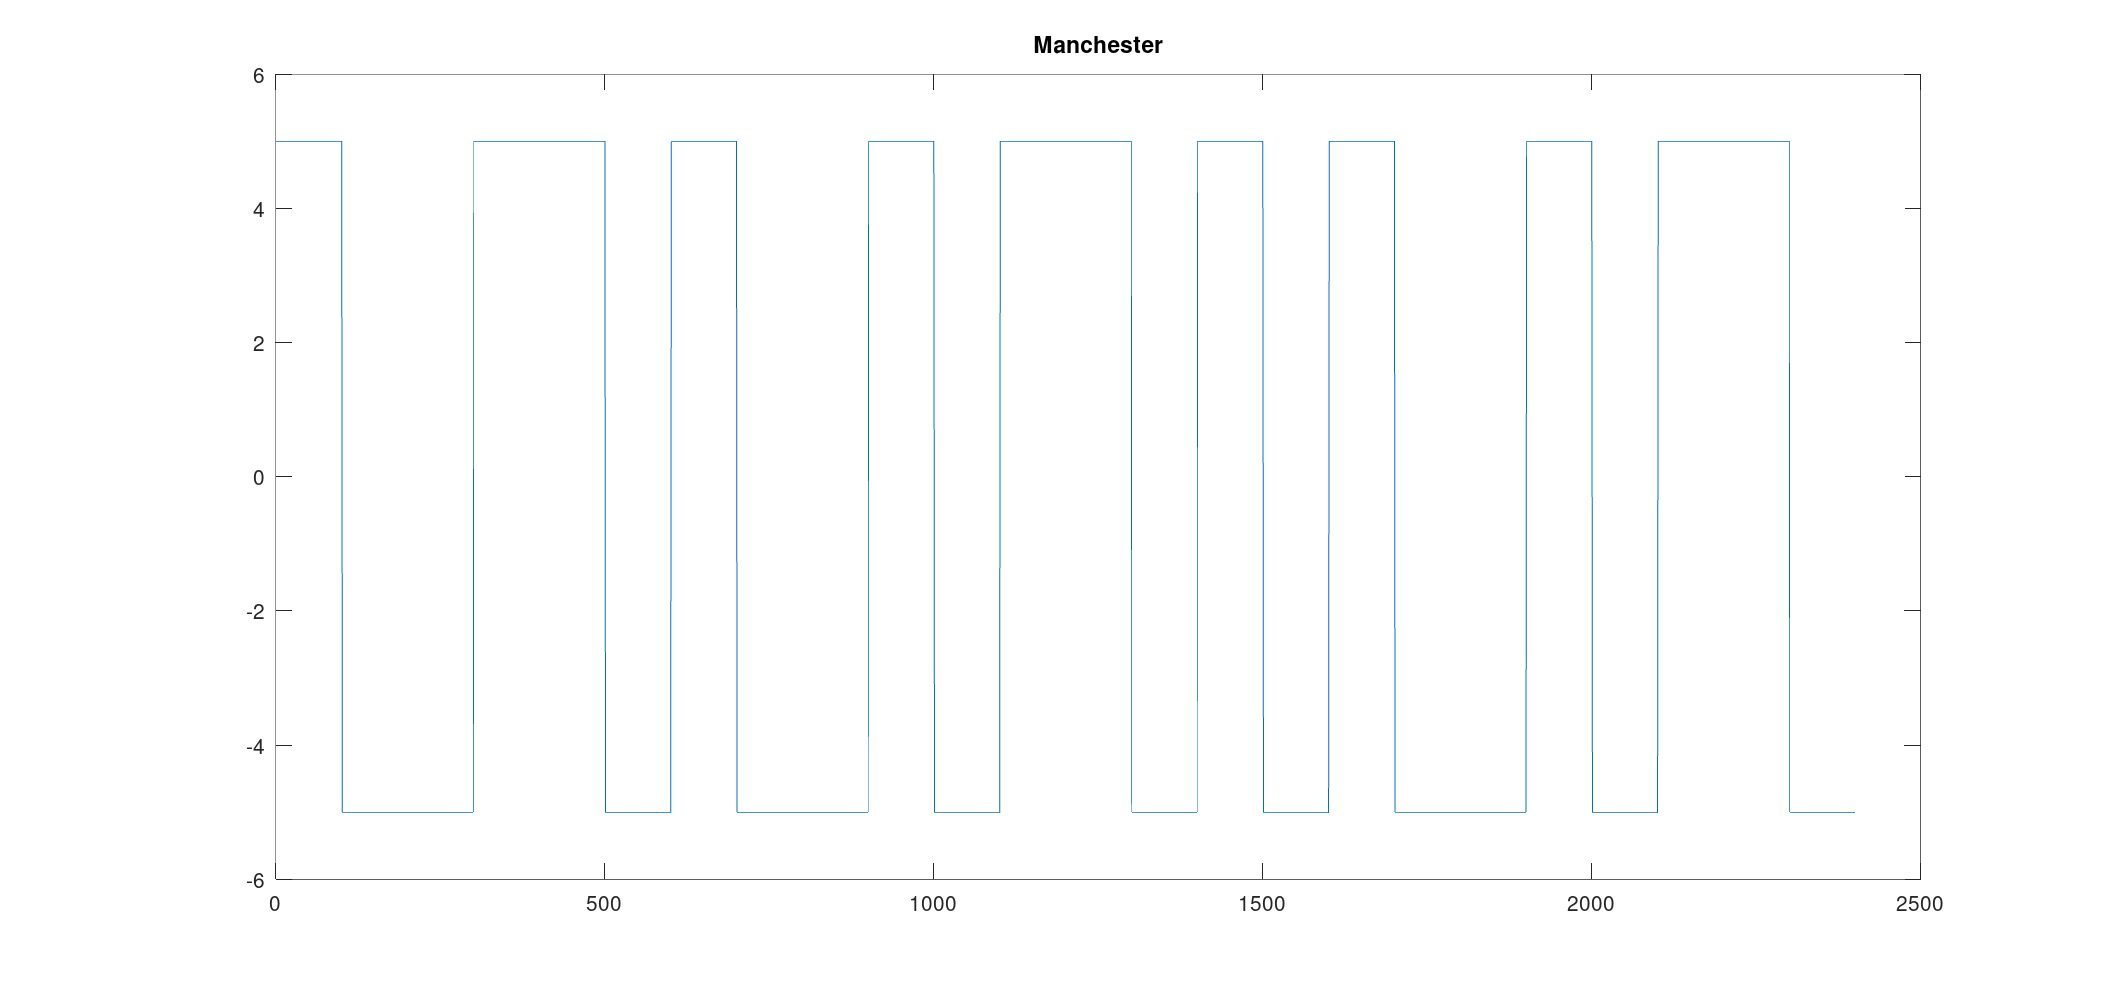
\includegraphics[width=0.7\textwidth]{../octave/coding/signal/manchester.png}
            \captionof{figure}{Манчестрерское кодирование.}
            \label{img:coding-sig-manchester}
        \end{center}
        \begin{center}
            \centering
            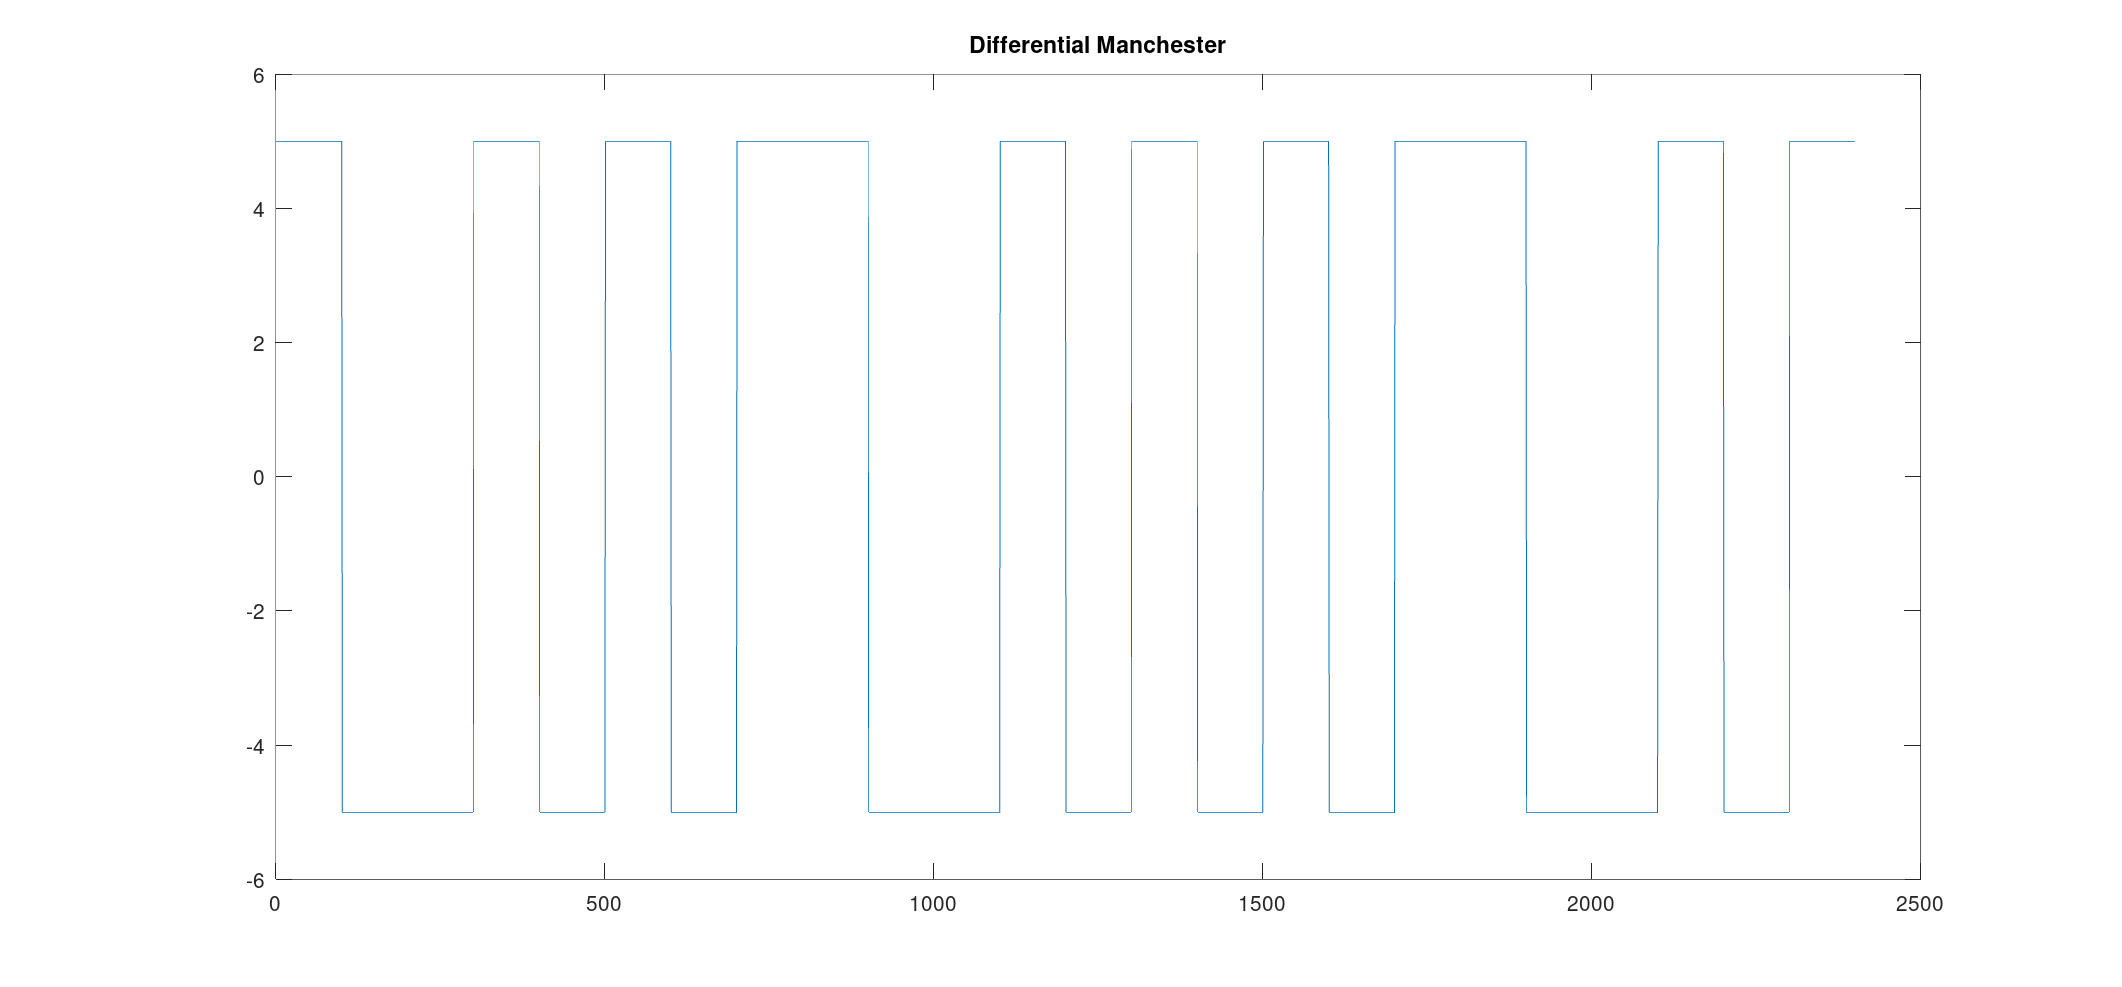
\includegraphics[width=0.7\textwidth]{../octave/coding/signal/diffmanc.png}
            \captionof{figure}{Дифференциальное манчестерское кодирование.}
            \label{img:coding-sig-diffmanc}
        \end{center}

        \begin{center}
            \centering
            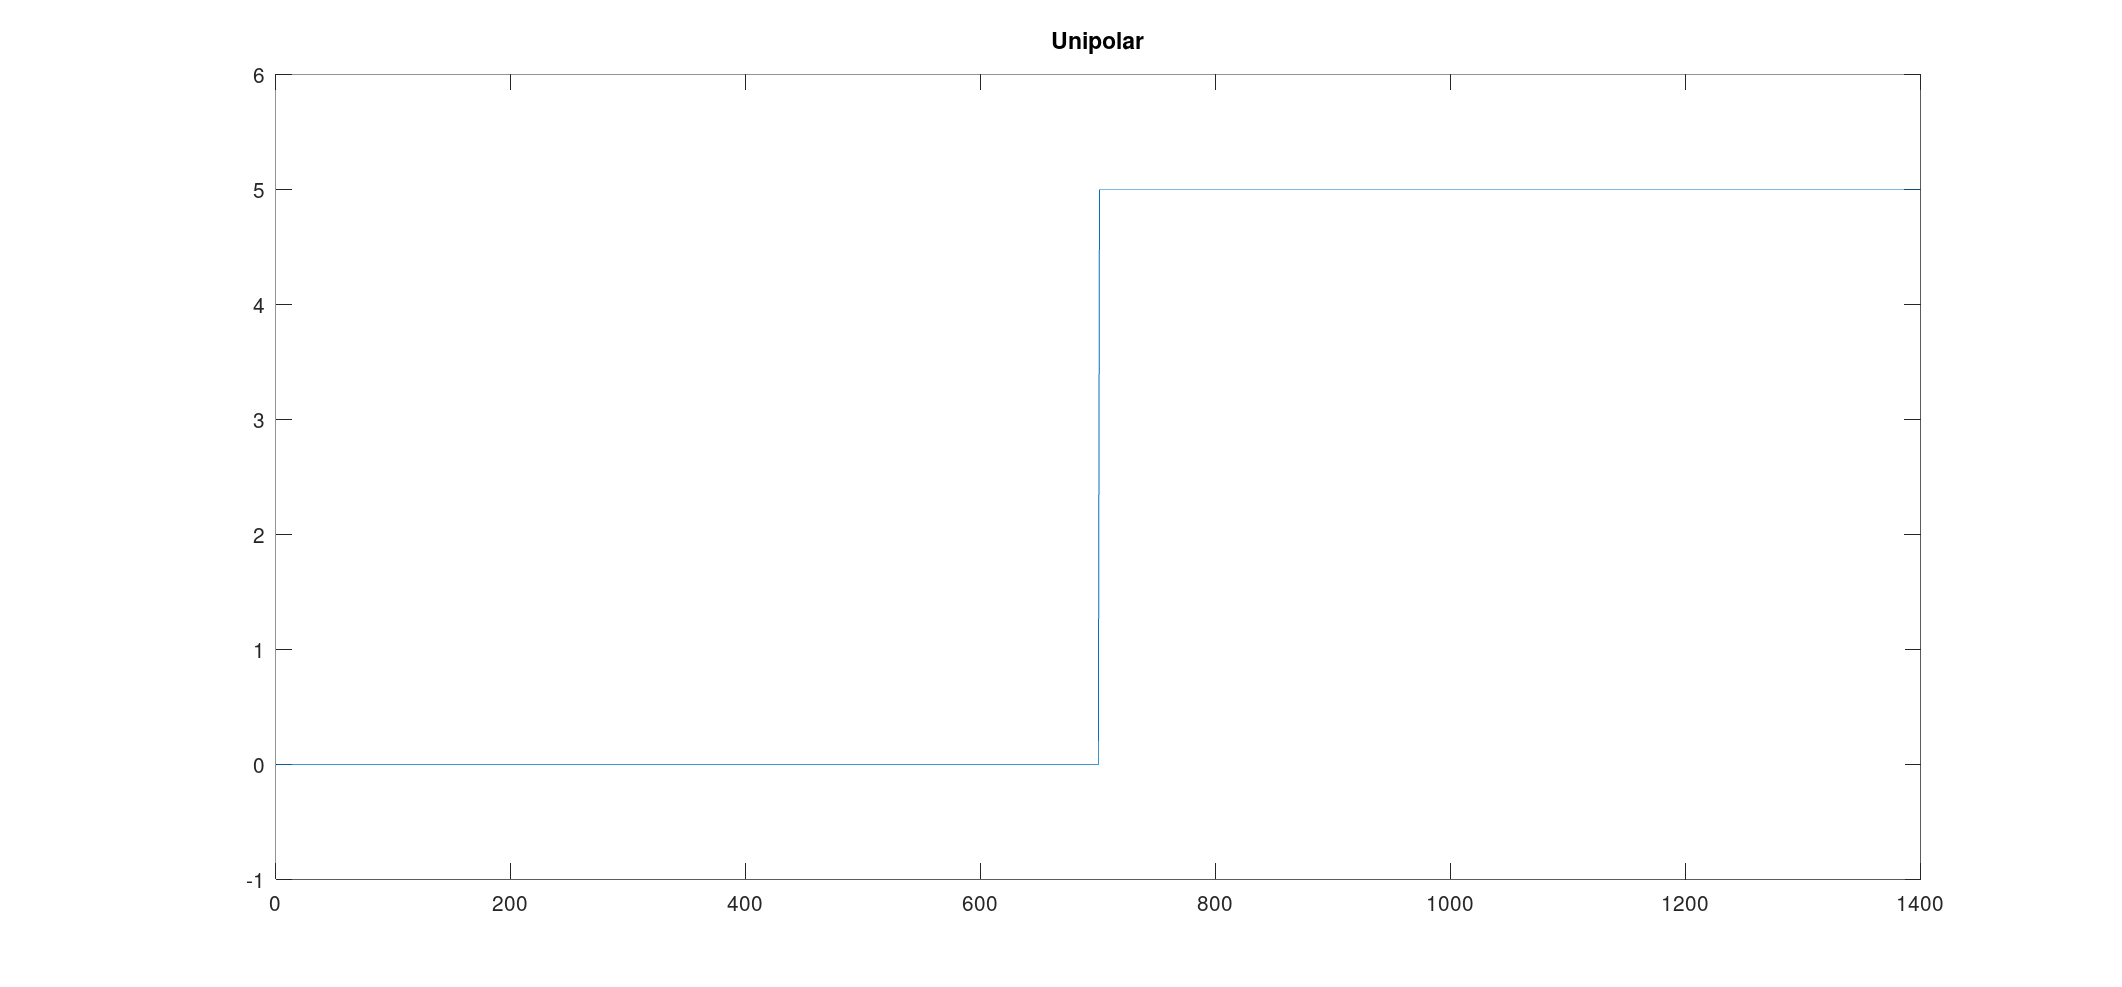
\includegraphics[width=0.7\textwidth]{../octave/coding/sync/unipolar.png}
            \captionof{figure}{Униполярное кодирование: нет синхронизации.}
            \label{img:coding-sync-unipolar}
        \end{center}
        \begin{center}
            \centering
            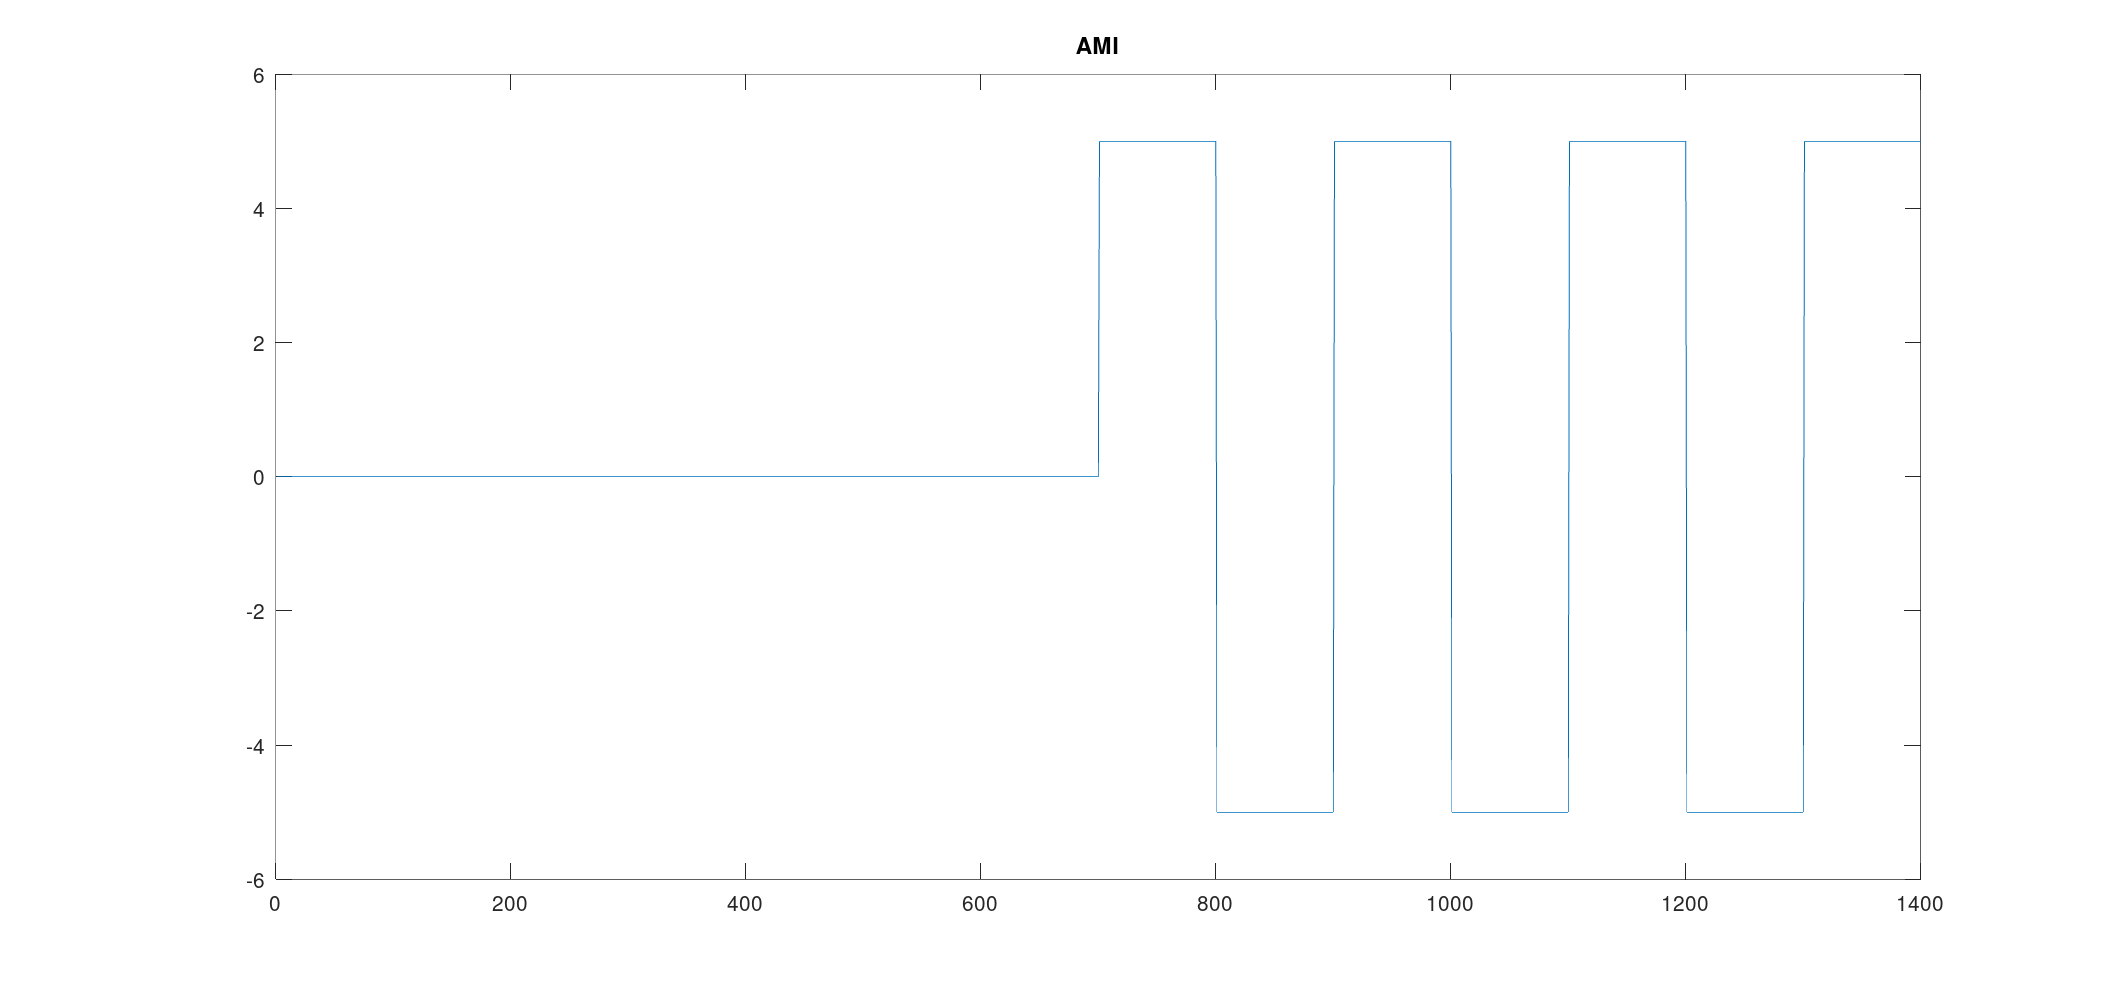
\includegraphics[width=0.7\textwidth]{../octave/coding/sync/ami.png}
            \captionof{figure}{Кодирование AMI: самосинхронизация при наличии сигнала.}
            \label{img:coding-sync-ami}
        \end{center}
        \begin{center}
            \centering
            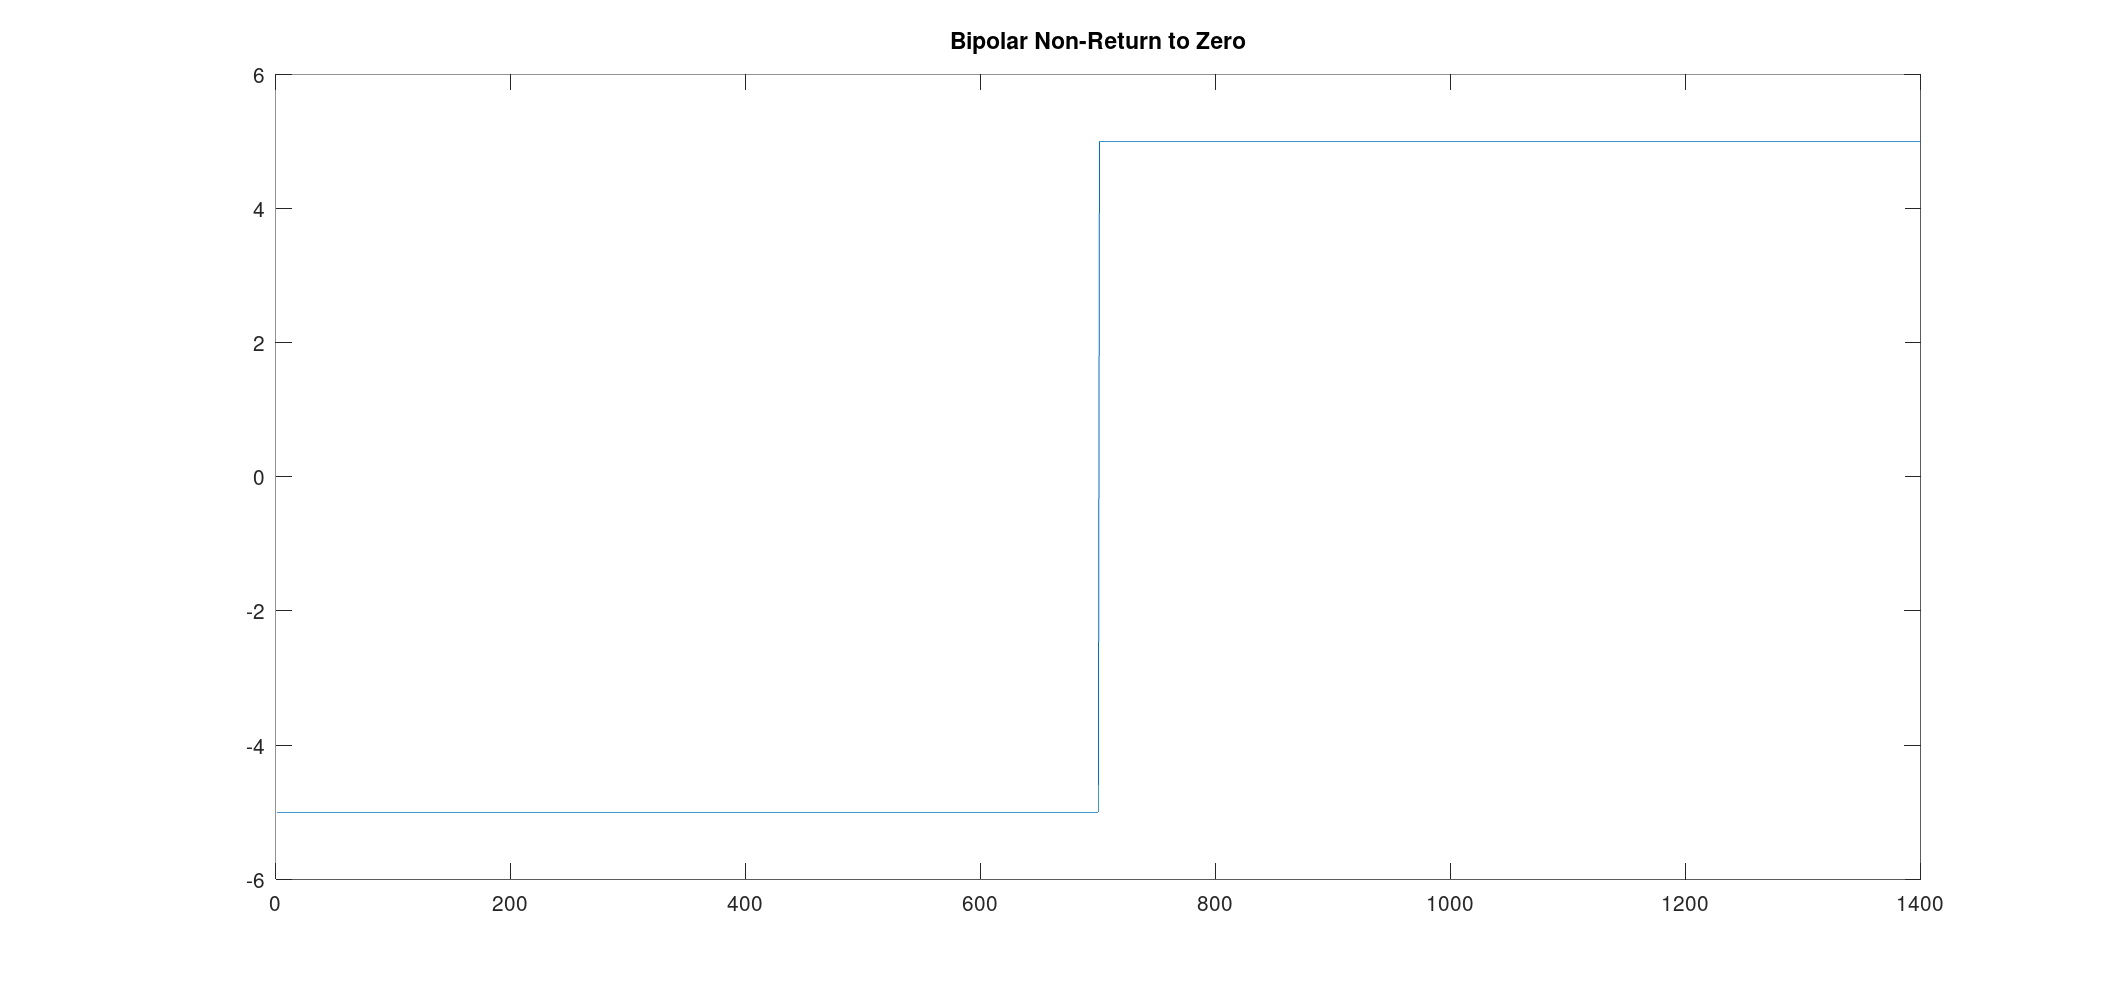
\includegraphics[width=0.7\textwidth]{../octave/coding/sync/bipolarnrz.png}
            \captionof{figure}{Кодирование NRZ: нет самосинхронизации.}
            \label{img:coding-sync-nrz}
        \end{center}
        \begin{center}
            \centering
            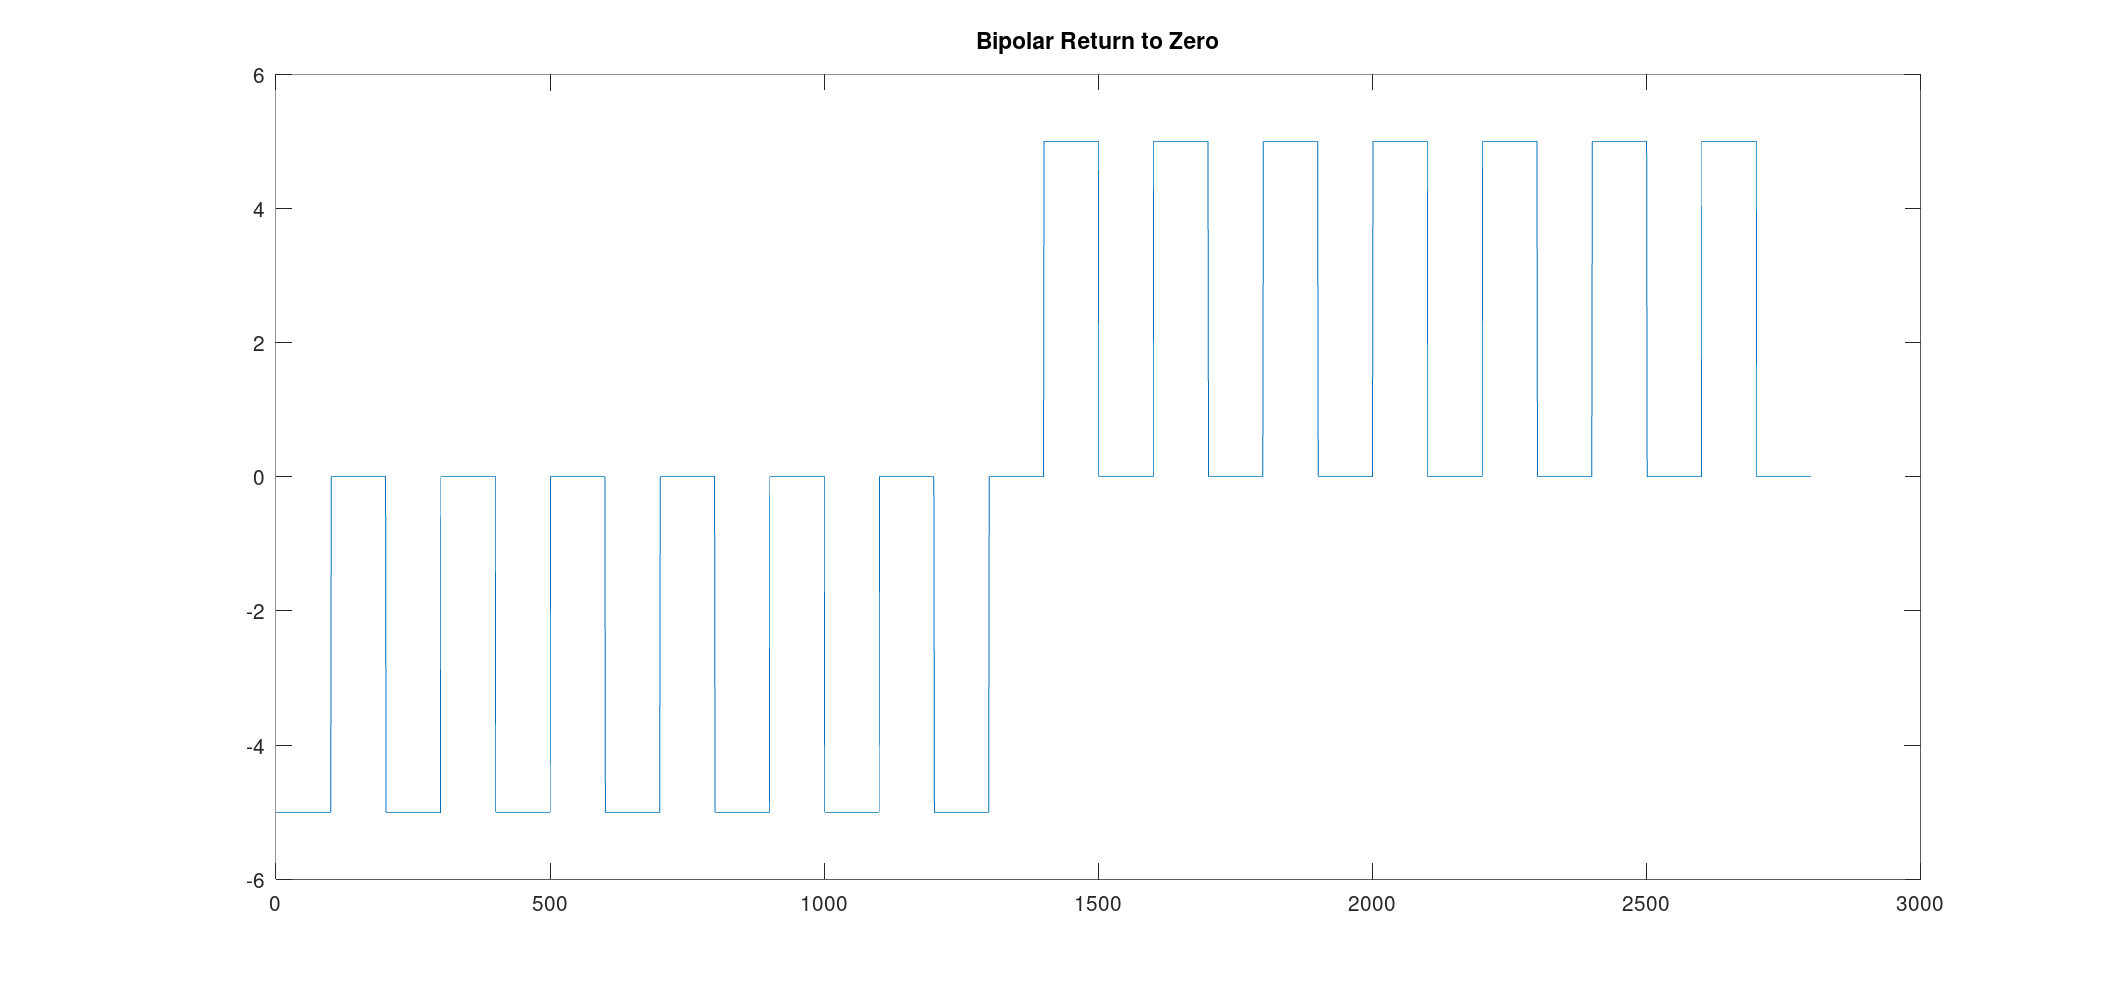
\includegraphics[width=0.7\textwidth]{../octave/coding/sync/bipolarrz.png}
            \captionof{figure}{Кодирование RZ: есть самосинхронизация}
            \label{img:coding-sync-rz}
        \end{center}
        \begin{center}
            \centering
            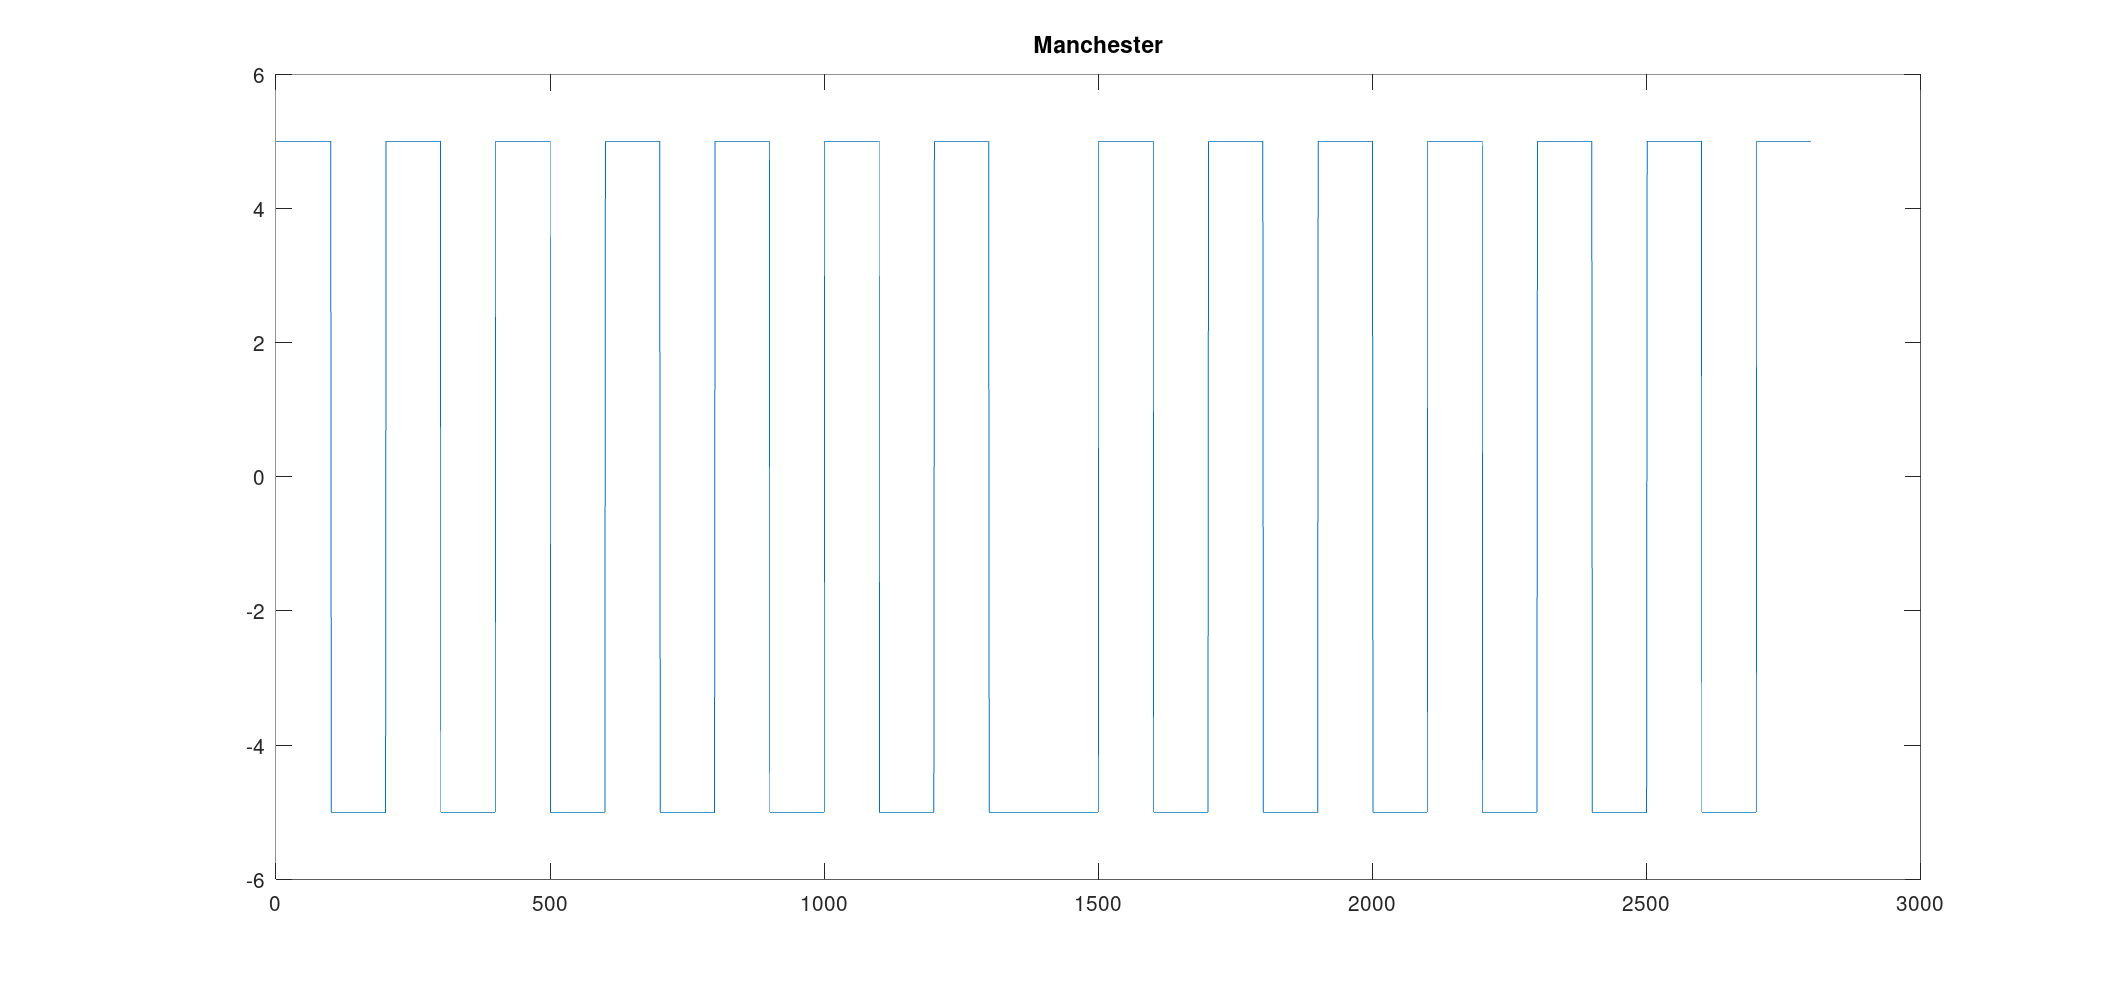
\includegraphics[width=0.7\textwidth]{../octave/coding/sync/manchester.png}
            \captionof{figure}{Манчестрерское кодирование: есть самосинхронизация}
            \label{img:coding-sync-manchester}
        \end{center}
        \begin{center}
            \centering
            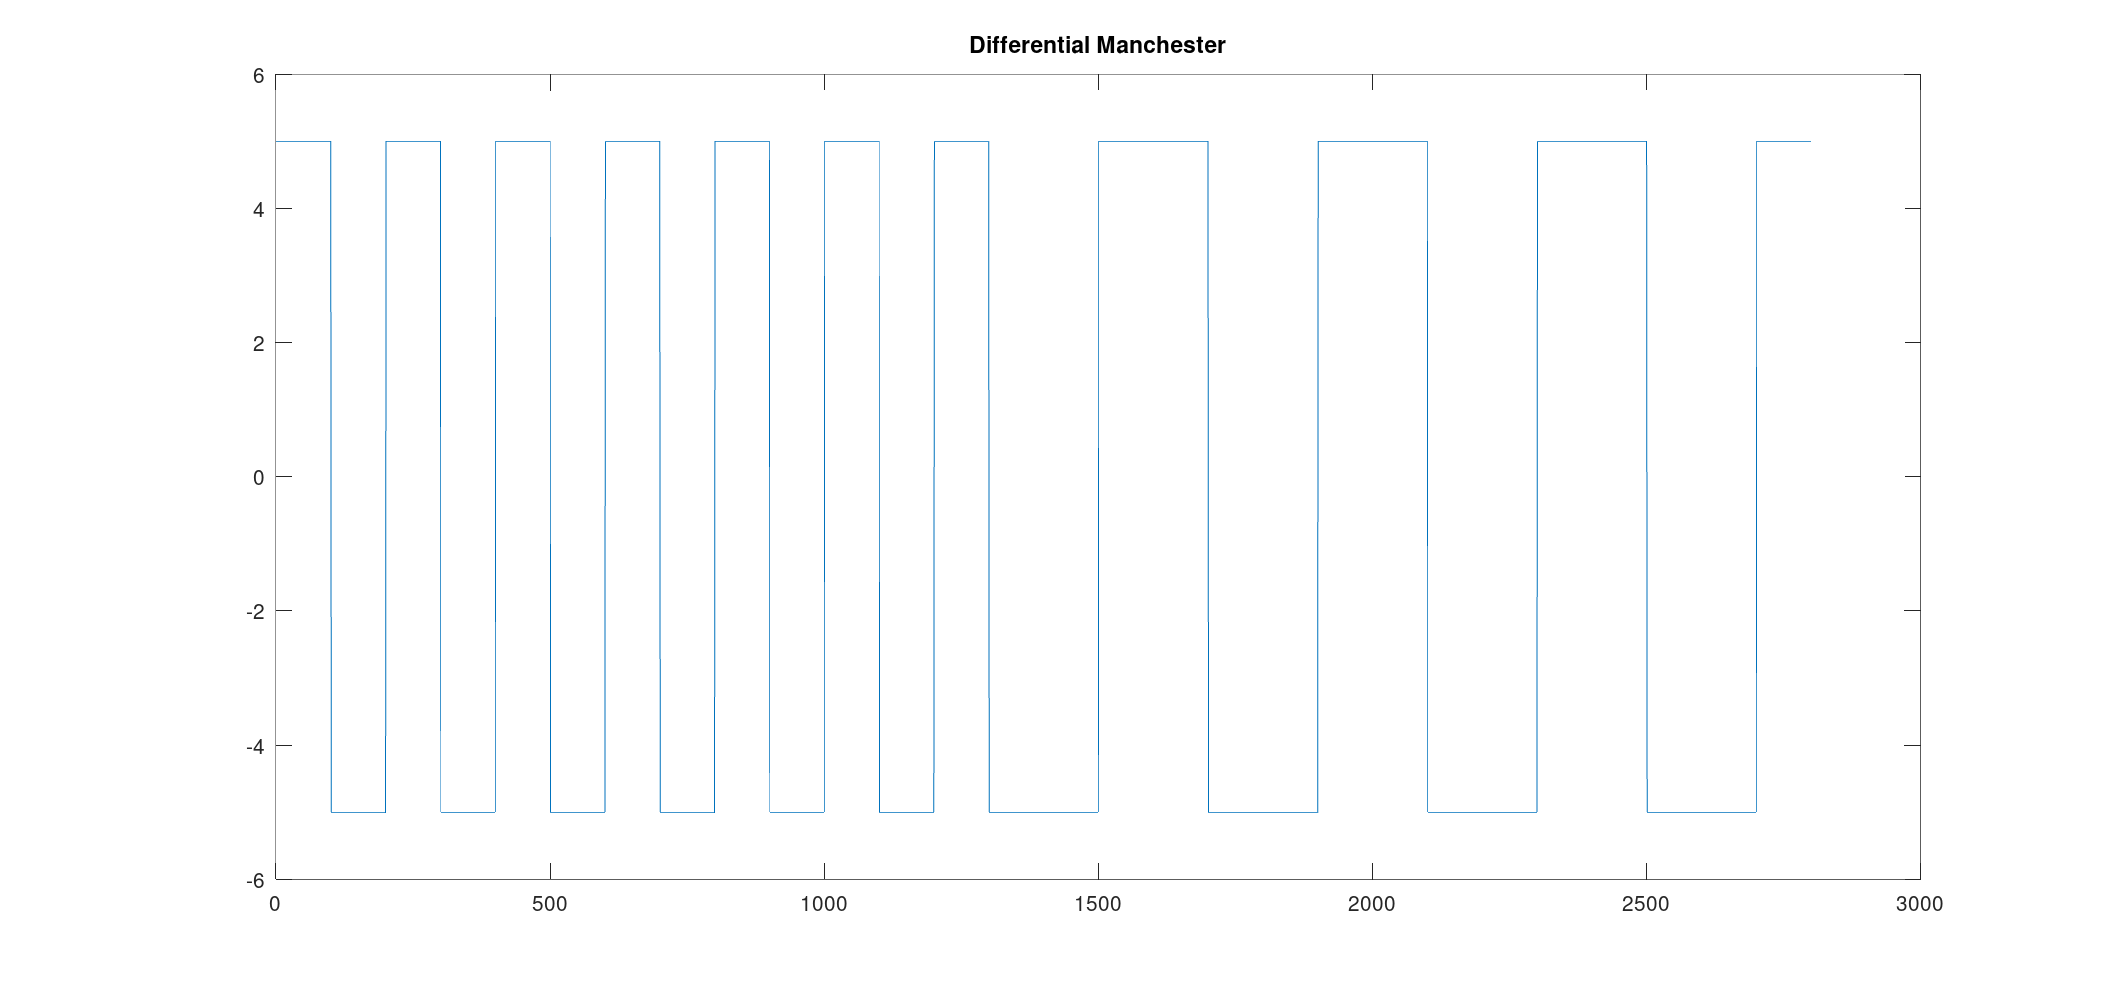
\includegraphics[width=0.7\textwidth]{../octave/coding/sync/diffmanc.png}
            \captionof{figure}{Дифференциальное манчестерское кодирование: есть самосинхронизация}
            \label{img:coding-sync-diffmanc}
        \end{center}

        \begin{center}
            \centering
            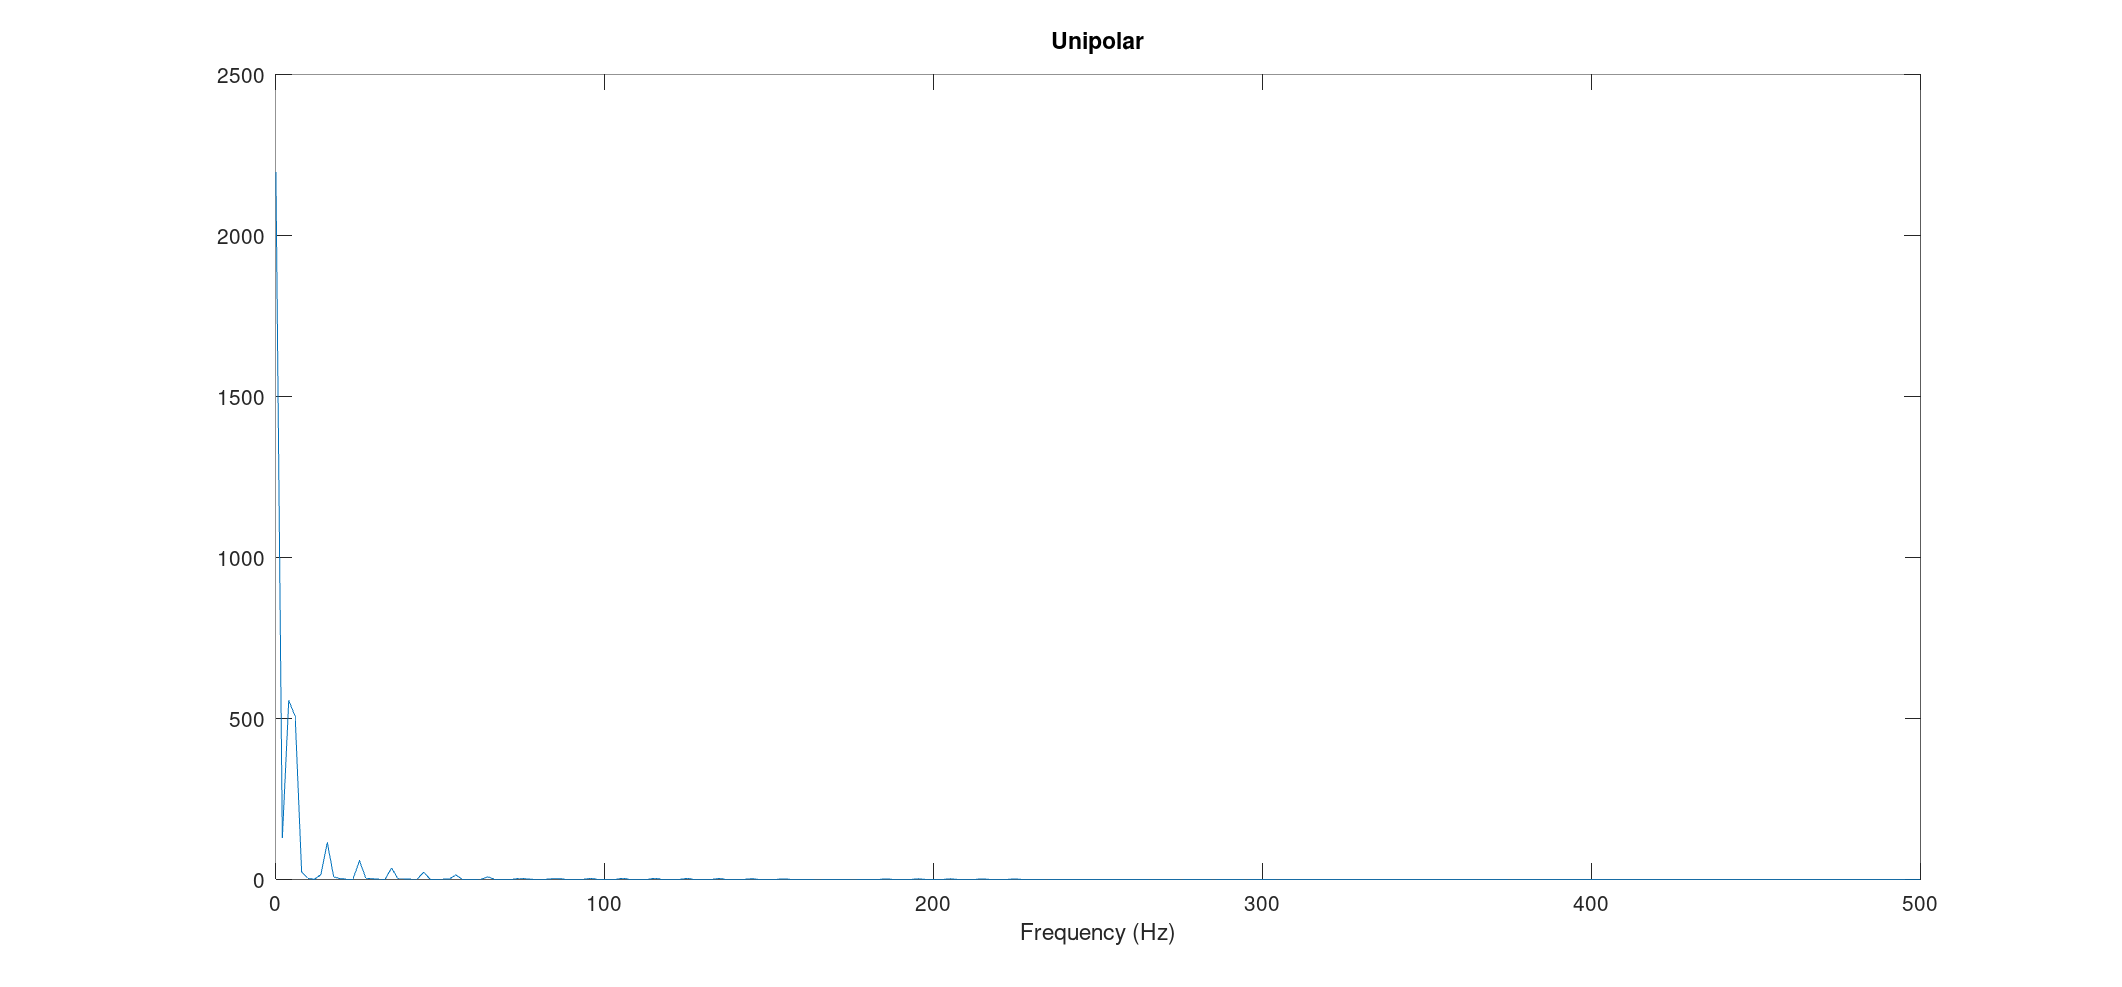
\includegraphics[width=0.7\textwidth]{../octave/coding/spectre/unipolar.png}
            \captionof{figure}{Униполярное кодирование: спектр сигнала}
            \label{img:coding-spectre-unipolar}
        \end{center}
        \begin{center}
            \centering
            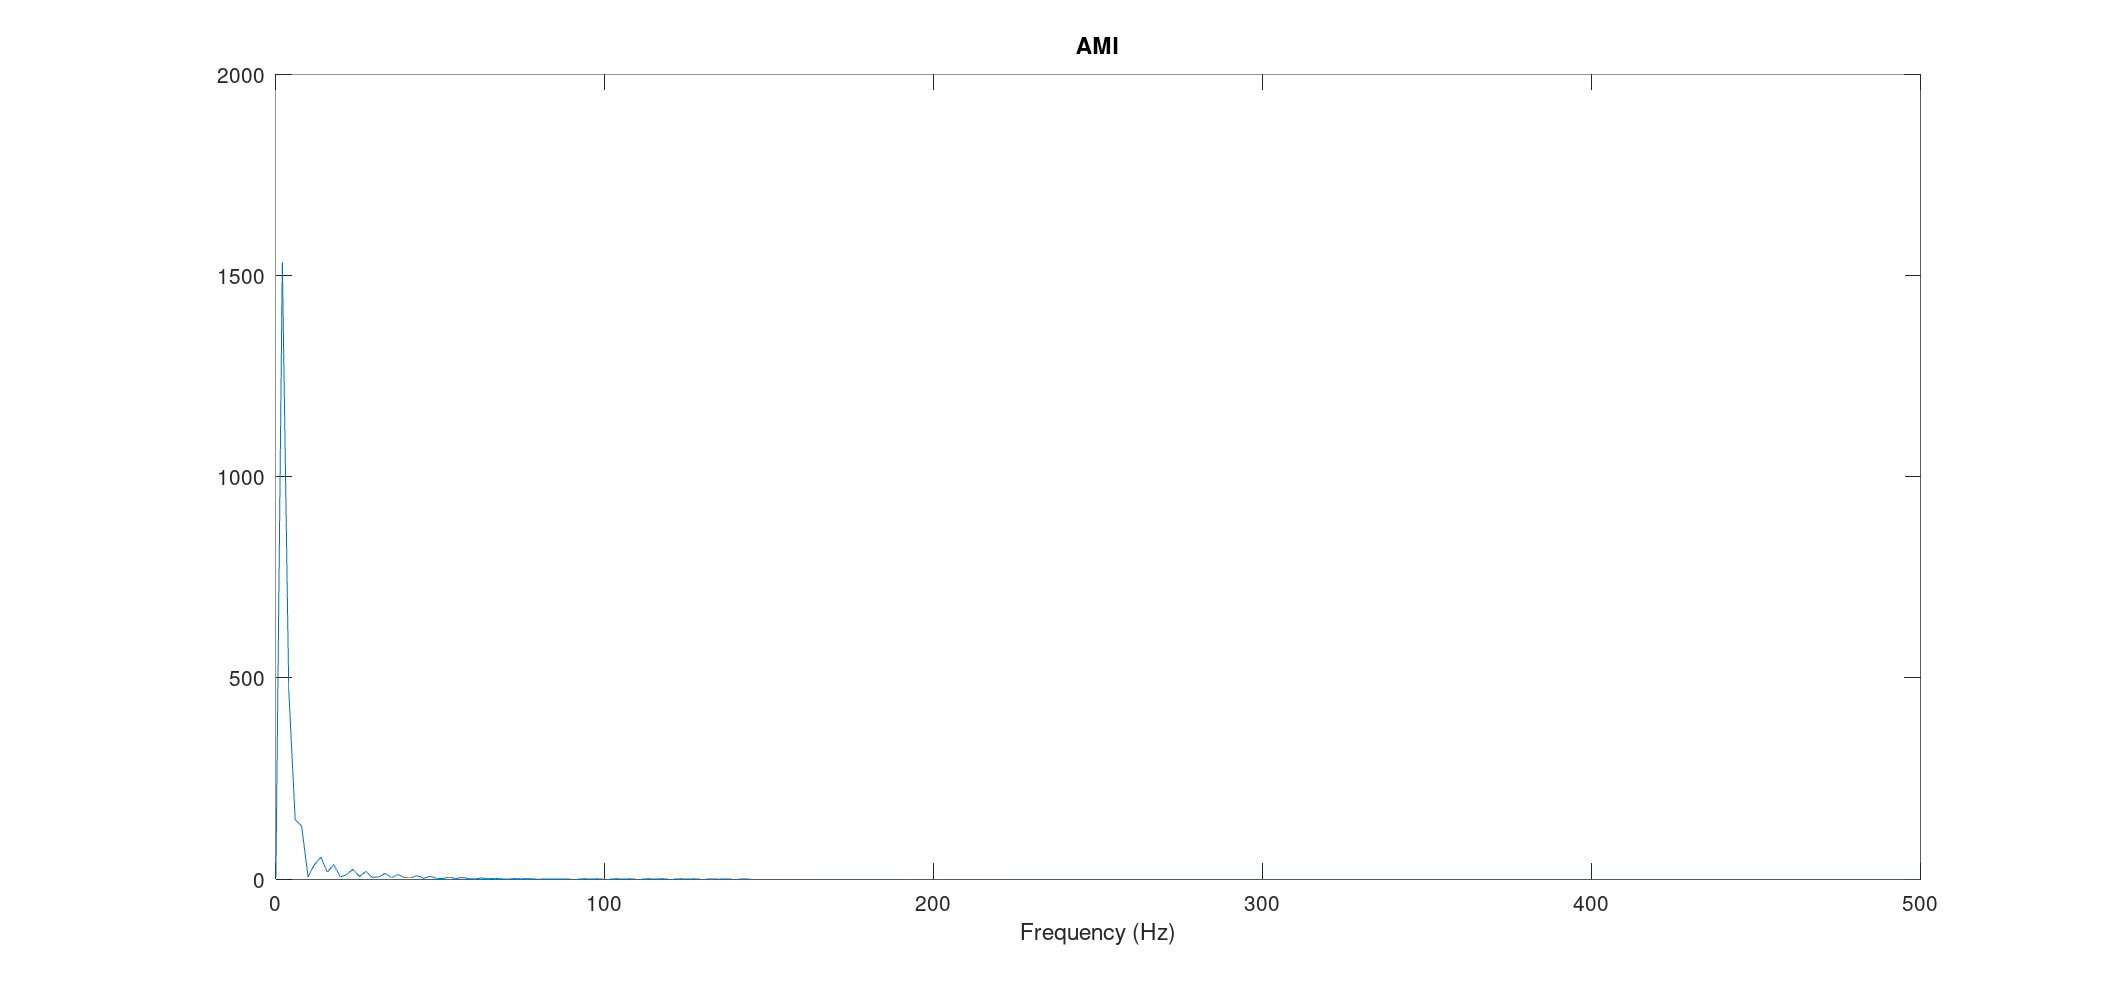
\includegraphics[width=0.7\textwidth]{../octave/coding/spectre/ami.png}
            \captionof{figure}{Кодирование AMI: спектр сигнала}
            \label{img:coding-spectre-ami}
        \end{center}
        \begin{center}
            \centering
            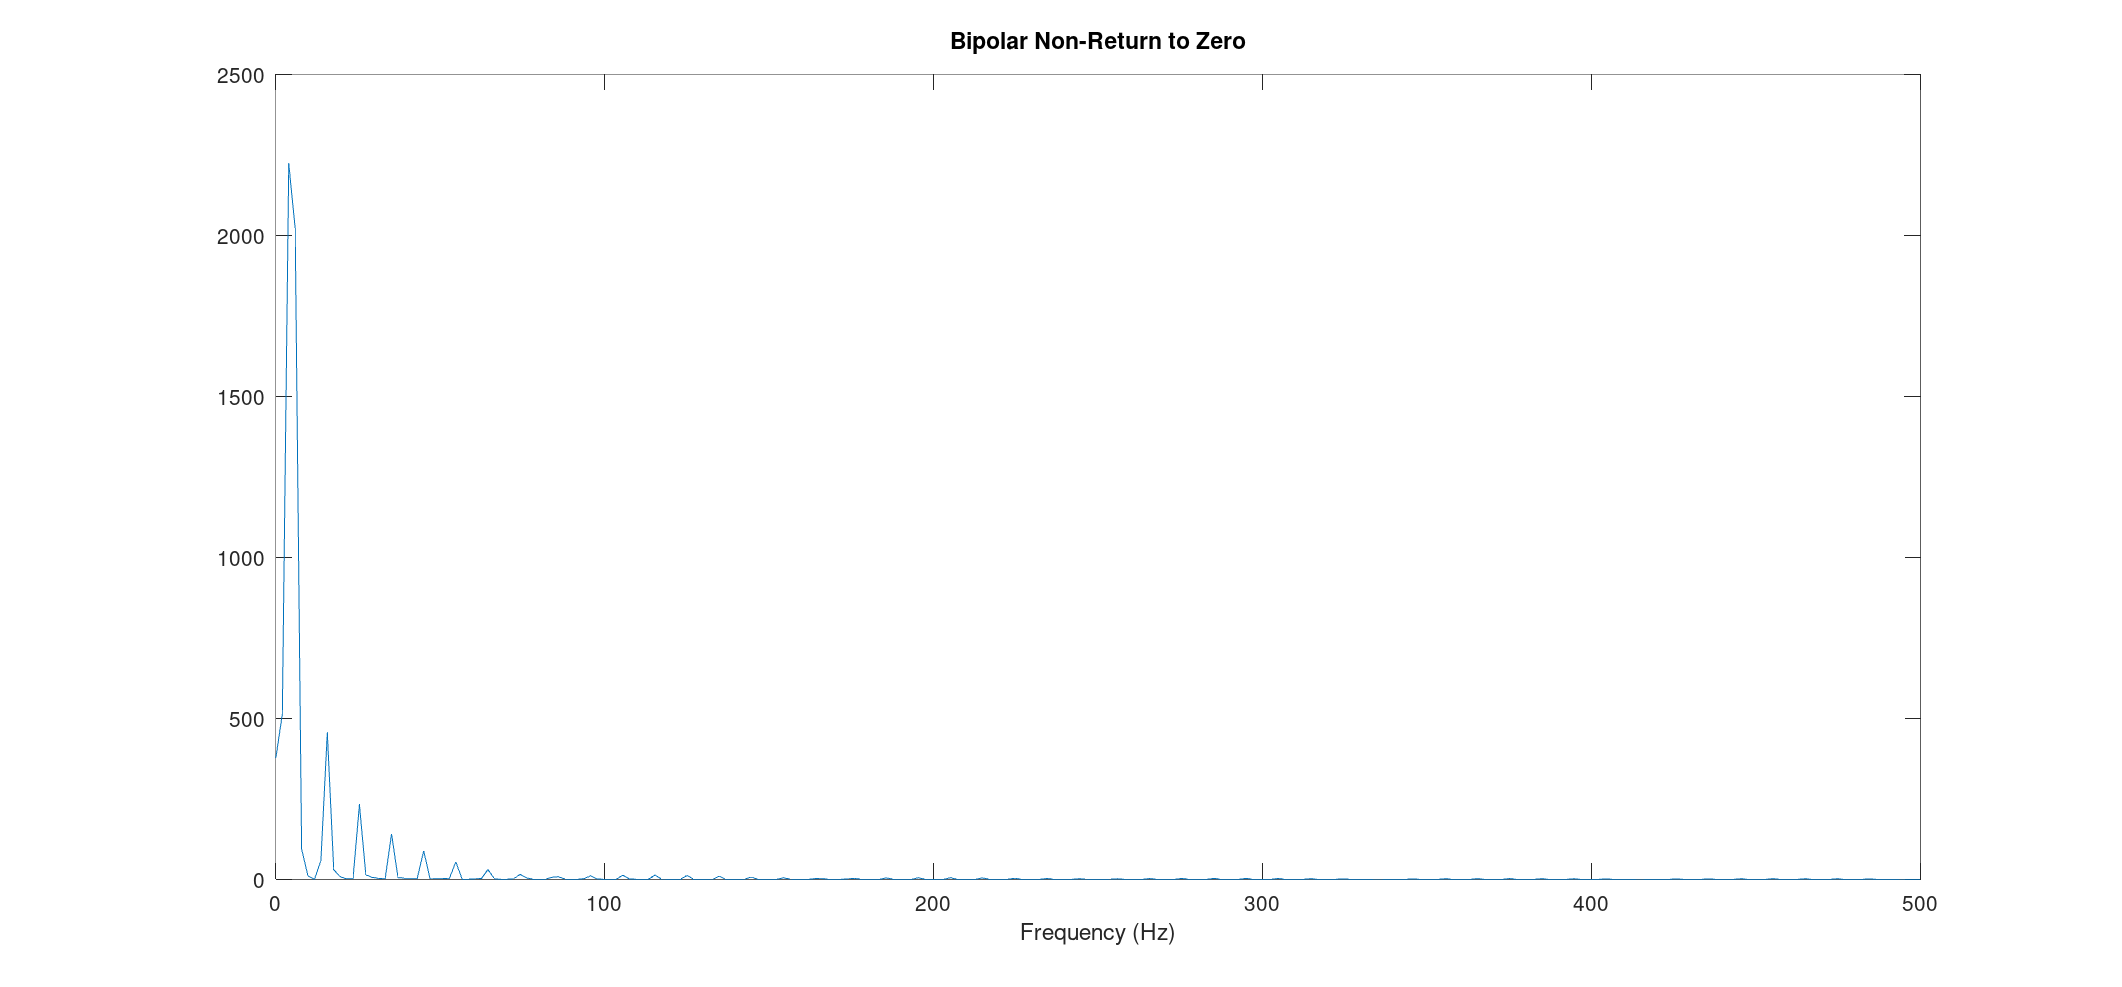
\includegraphics[width=0.7\textwidth]{../octave/coding/spectre/bipolarnrz.png}
            \captionof{figure}{Кодирование NRZ: спектр сигнала}
            \label{img:coding-spectre-nrz}
        \end{center}
        \begin{center}
            \centering
            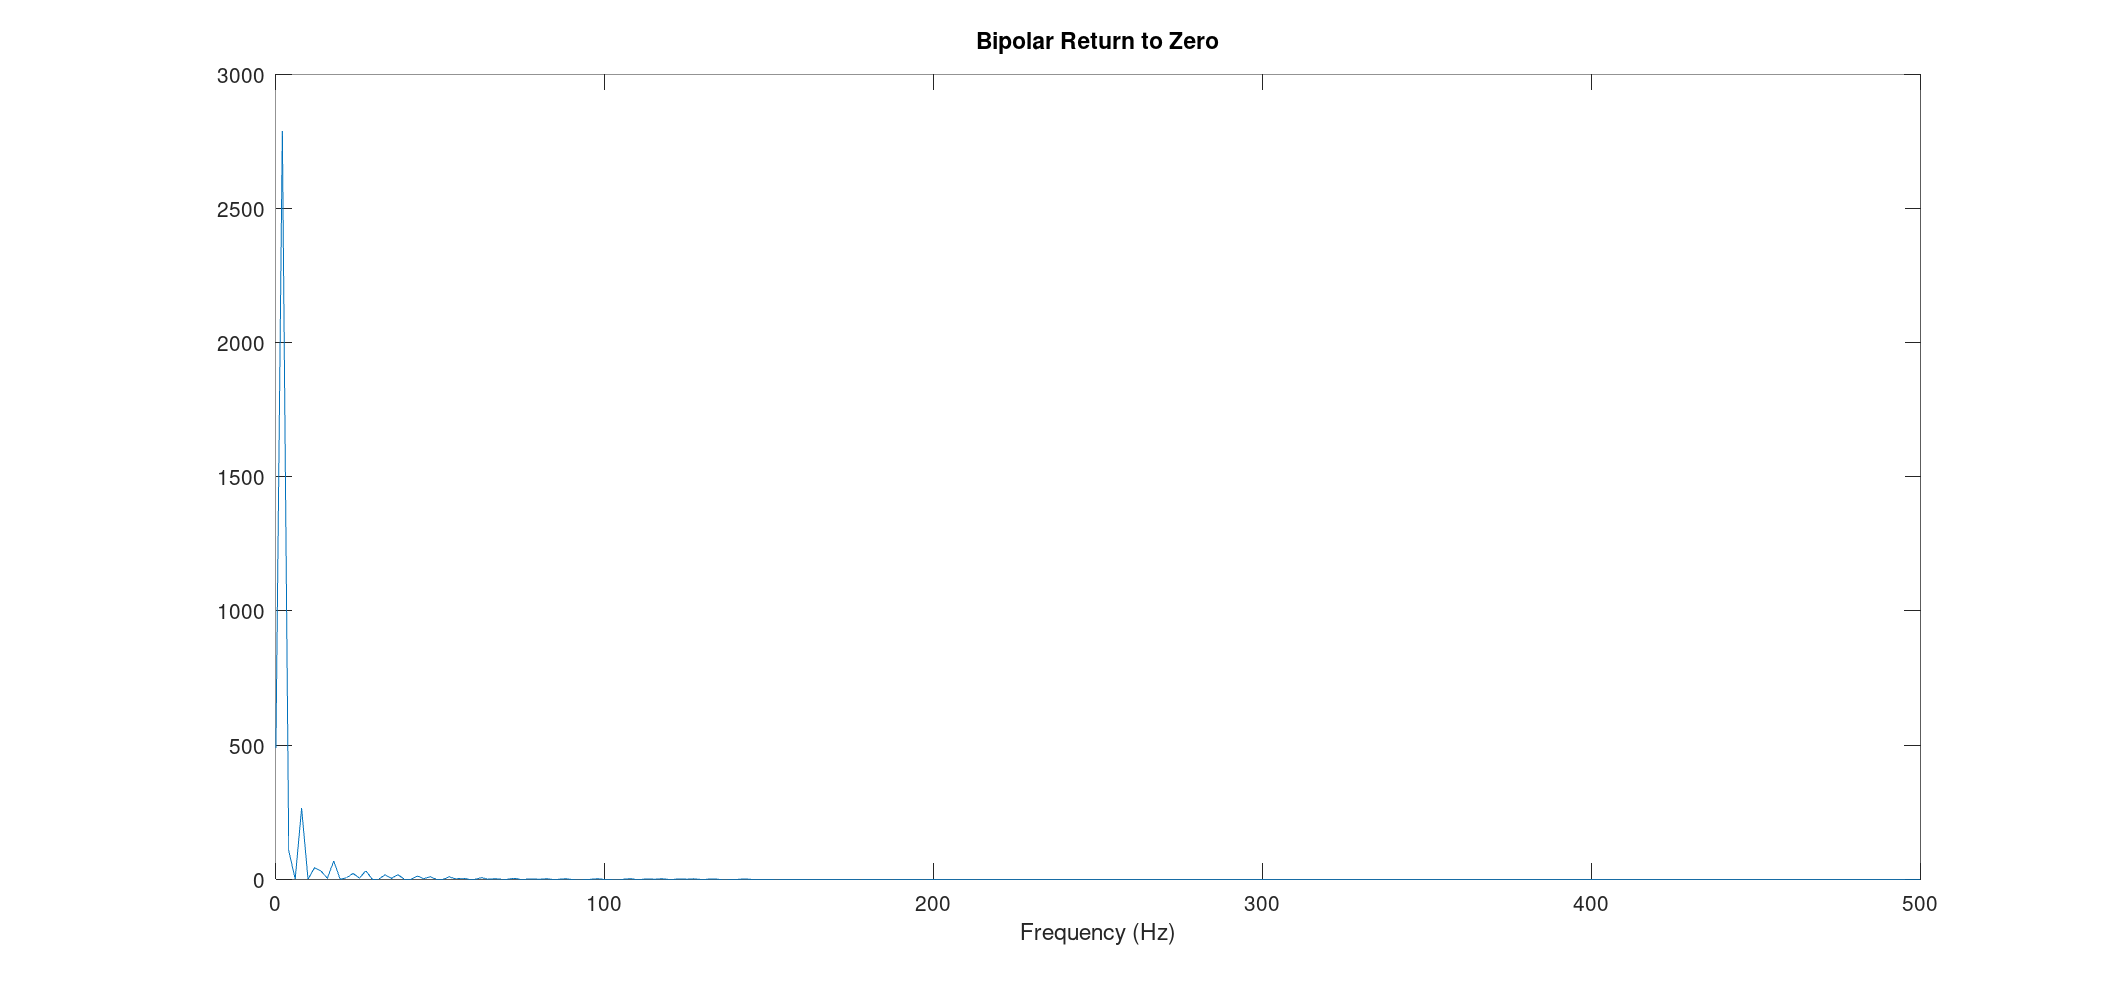
\includegraphics[width=0.7\textwidth]{../octave/coding/spectre/bipolarrz.png}
            \captionof{figure}{Кодирование RZ: спектр сигнала}
            \label{img:coding-spectre-rz}
        \end{center}
        \begin{center}
            \centering
            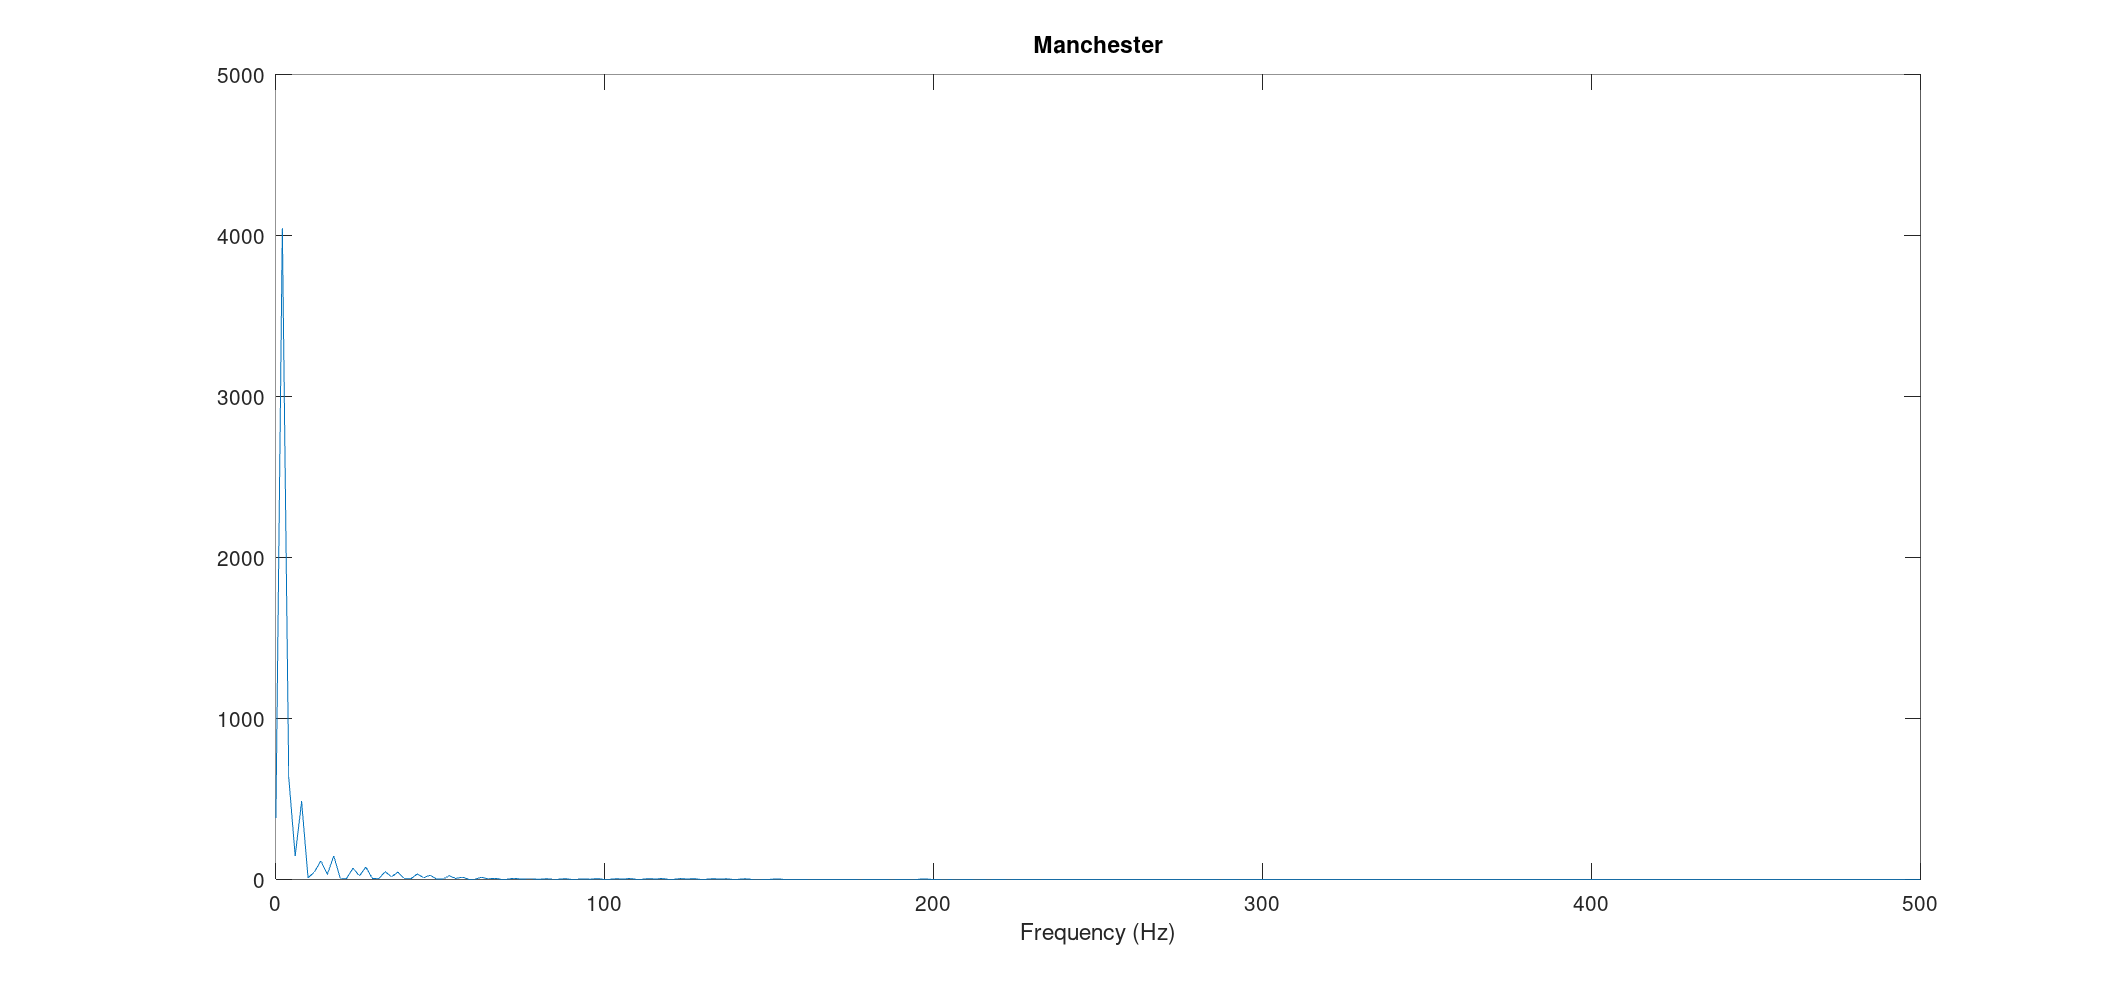
\includegraphics[width=0.7\textwidth]{../octave/coding/spectre/manchester.png}
            \captionof{figure}{Манчестрерское кодирование: спектр сигнала}
            \label{img:coding-spectre-manchester}
        \end{center}
        \begin{center}
            \centering
            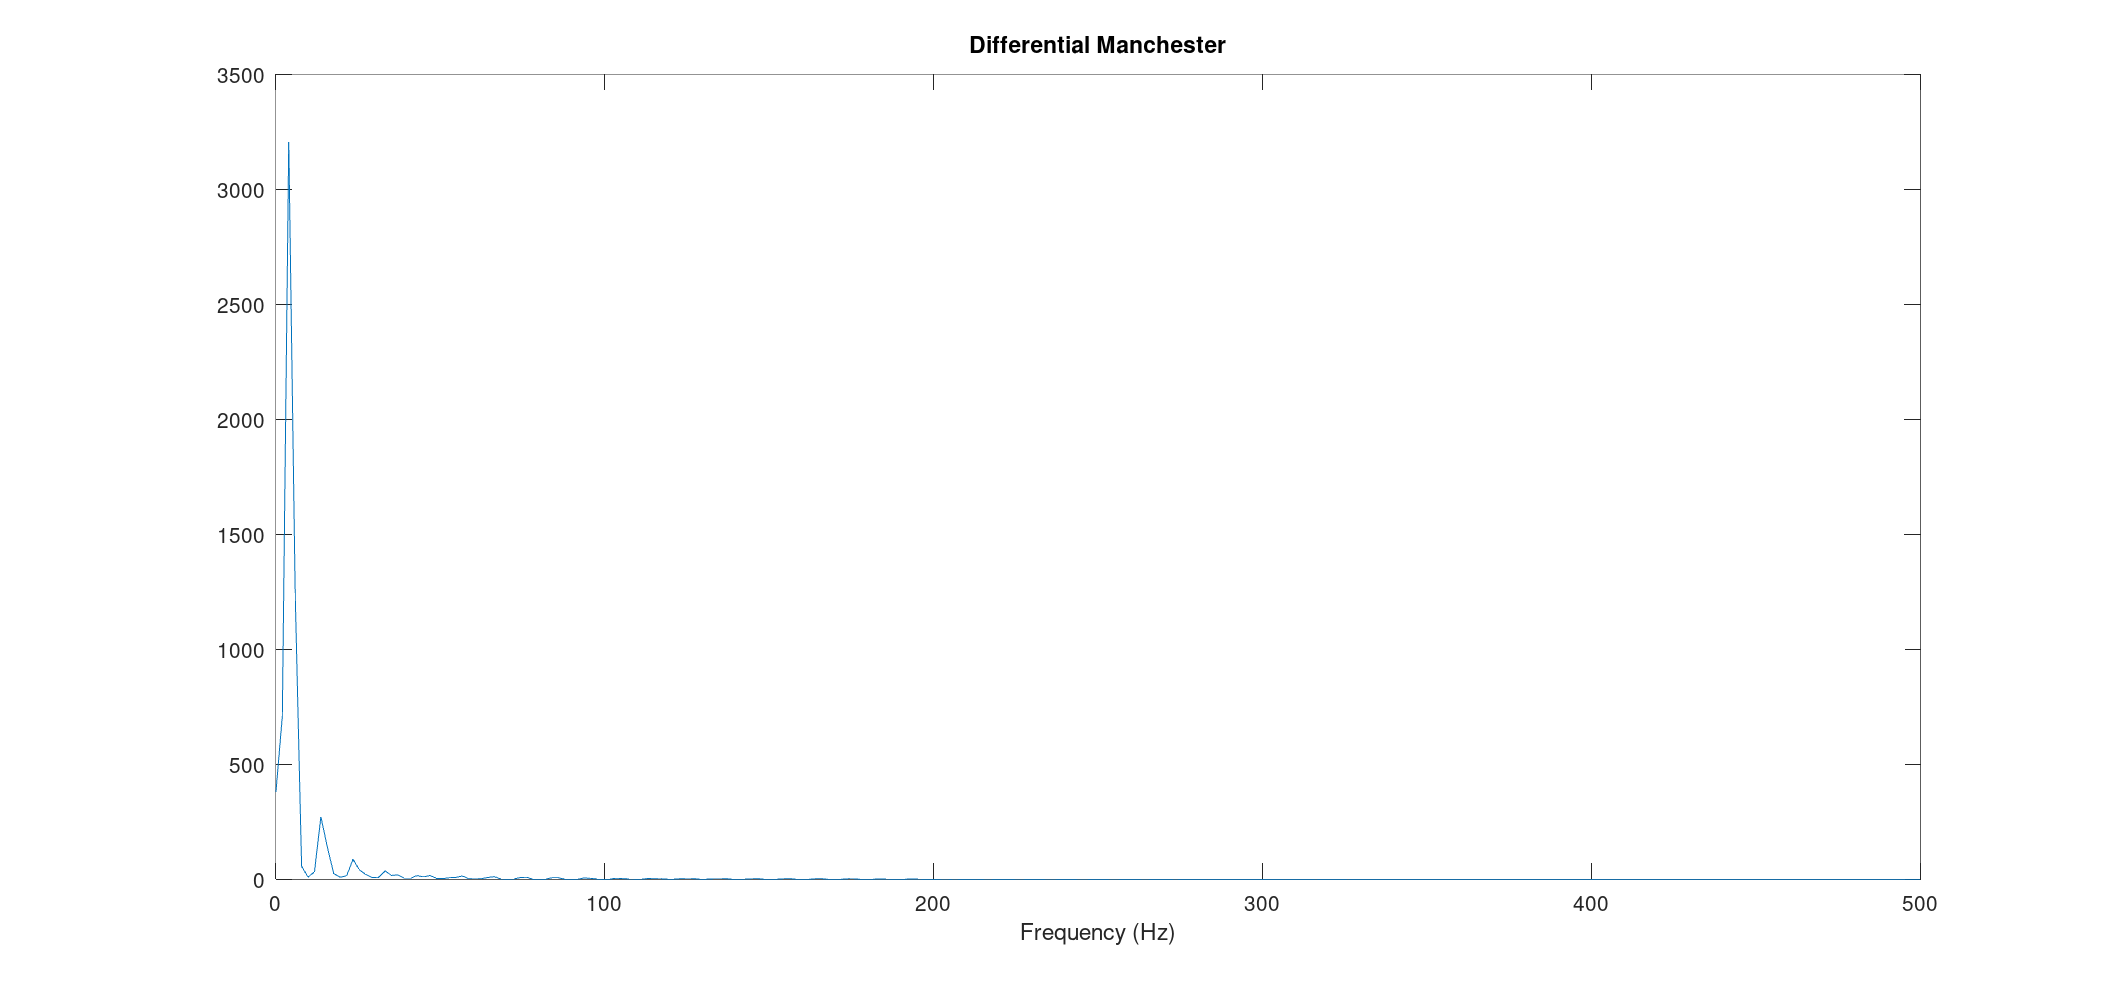
\includegraphics[width=0.7\textwidth]{../octave/coding/spectre/diffmanc.png}
            \captionof{figure}{Дифференциальное манчестерское кодирование: спектр сигнала}
            \label{img:coding-spectre-diffmanc}
        \end{center}

\end{enumerate}

\section{Выводы}
В рамках выполнения лабораторной работы изучили методы кодирования и модуляции
сигналов с помощью высокоуровнего языка программирования Octave, в том числе
познакомились с принципами модуляции сигнала на примере аналоговй амплитудной
модуляции, исследовали свойства самосинхронизации сигнала.
\end{document}
